\documentclass[twoside]{book}

% Packages required by doxygen
\usepackage{calc}
\usepackage{doxygen}
\usepackage{graphicx}
\usepackage[utf8]{inputenc}
\usepackage{makeidx}
\usepackage{multicol}
\usepackage{multirow}
\usepackage{textcomp}
\usepackage[table]{xcolor}

% Font selection
\usepackage[T1]{fontenc}
\usepackage{mathptmx}
\usepackage[scaled=.90]{helvet}
\usepackage{courier}
\usepackage{amssymb}
\usepackage{sectsty}
\renewcommand{\familydefault}{\sfdefault}
\allsectionsfont{%
  \fontseries{bc}\selectfont%
  \color{darkgray}%
}
\renewcommand{\DoxyLabelFont}{%
  \fontseries{bc}\selectfont%
  \color{darkgray}%
}
\newcommand{\+}{\discretionary{\mbox{\scriptsize$\hookleftarrow$}}{}{}}

% Page & text layout
\usepackage{geometry}
\geometry{%
  a4paper,%
  top=2.5cm,%
  bottom=2.5cm,%
  left=2.5cm,%
  right=2.5cm%
}
\tolerance=750
\hfuzz=15pt
\hbadness=750
\setlength{\emergencystretch}{15pt}
\setlength{\parindent}{0cm}
\setlength{\parskip}{0.2cm}
\makeatletter
\renewcommand{\paragraph}{%
  \@startsection{paragraph}{4}{0ex}{-1.0ex}{1.0ex}{%
    \normalfont\normalsize\bfseries\SS@parafont%
  }%
}
\renewcommand{\subparagraph}{%
  \@startsection{subparagraph}{5}{0ex}{-1.0ex}{1.0ex}{%
    \normalfont\normalsize\bfseries\SS@subparafont%
  }%
}
\makeatother

% Headers & footers
\usepackage{fancyhdr}
\pagestyle{fancyplain}
\fancyhead[LE]{\fancyplain{}{\bfseries\thepage}}
\fancyhead[CE]{\fancyplain{}{}}
\fancyhead[RE]{\fancyplain{}{\bfseries\leftmark}}
\fancyhead[LO]{\fancyplain{}{\bfseries\rightmark}}
\fancyhead[CO]{\fancyplain{}{}}
\fancyhead[RO]{\fancyplain{}{\bfseries\thepage}}
\fancyfoot[LE]{\fancyplain{}{}}
\fancyfoot[CE]{\fancyplain{}{}}
\fancyfoot[RE]{\fancyplain{}{\bfseries\scriptsize Generated on Tue Mar 4 2014 09\+:57\+:27 for Clear\+Blade i\+O\+S S\+D\+K by Doxygen }}
\fancyfoot[LO]{\fancyplain{}{\bfseries\scriptsize Generated on Tue Mar 4 2014 09\+:57\+:27 for Clear\+Blade i\+O\+S S\+D\+K by Doxygen }}
\fancyfoot[CO]{\fancyplain{}{}}
\fancyfoot[RO]{\fancyplain{}{}}
\renewcommand{\footrulewidth}{0.4pt}
\renewcommand{\chaptermark}[1]{%
  \markboth{#1}{}%
}
\renewcommand{\sectionmark}[1]{%
  \markright{\thesection\ #1}%
}

% Indices & bibliography
\usepackage{natbib}
\usepackage[titles]{tocloft}
\setcounter{tocdepth}{3}
\setcounter{secnumdepth}{5}
\makeindex

% Hyperlinks (required, but should be loaded last)
\usepackage{ifpdf}
\ifpdf
  \usepackage[pdftex,pagebackref=true]{hyperref}
\else
  \usepackage[ps2pdf,pagebackref=true]{hyperref}
\fi
\hypersetup{%
  colorlinks=true,%
  linkcolor=blue,%
  citecolor=blue,%
  unicode%
}

% Custom commands
\newcommand{\clearemptydoublepage}{%
  \newpage{\pagestyle{empty}\cleardoublepage}%
}


%===== C O N T E N T S =====

\begin{document}

% Titlepage & ToC
\hypersetup{pageanchor=false,
             bookmarks=true,
             bookmarksnumbered=true,
             pdfencoding=unicode
            }
\pagenumbering{roman}
\begin{titlepage}
\vspace*{7cm}
\begin{center}%
{\Large Clear\+Blade i\+O\+S S\+D\+K }\\
\vspace*{1cm}
{\large Generated by Doxygen 1.8.6}\\
\vspace*{0.5cm}
{\small Tue Mar 4 2014 09:57:27}\\
\end{center}
\end{titlepage}
\clearemptydoublepage
\tableofcontents
\clearemptydoublepage
\pagenumbering{arabic}
\hypersetup{pageanchor=true}

%--- Begin generated contents ---
\chapter{Hierarchical Index}
\section{Class Hierarchy}
This inheritance list is sorted roughly, but not completely, alphabetically\-:\begin{DoxyCompactList}
\item A\-F\-H\-T\-T\-P\-Client\begin{DoxyCompactList}
\item \contentsline{section}{C\-B\-H\-T\-T\-P\-Client}{\pageref{interface_c_b_h_t_t_p_client}}{}
\end{DoxyCompactList}
\item \contentsline{section}{C\-B\-Message\-Client()}{\pageref{category_c_b_message_client_07_08}}{}
\item N\-S\-Object\begin{DoxyCompactList}
\item \contentsline{section}{C\-B\-Collection}{\pageref{interface_c_b_collection}}{}
\item \contentsline{section}{C\-B\-Item}{\pageref{interface_c_b_item}}{}
\item \contentsline{section}{C\-B\-Message}{\pageref{interface_c_b_message}}{}
\item \contentsline{section}{C\-B\-Message\-Client}{\pageref{interface_c_b_message_client}}{}
\item \contentsline{section}{C\-B\-Query}{\pageref{interface_c_b_query}}{}
\item \contentsline{section}{Clear\-Blade}{\pageref{interface_clear_blade}}{}
\end{DoxyCompactList}
\item $<$N\-S\-Object$>$\begin{DoxyCompactList}
\item \contentsline{section}{$<$C\-B\-Message\-Client\-Delegate$>$}{\pageref{protocol_c_b_message_client_delegate-p}}{}
\end{DoxyCompactList}
\end{DoxyCompactList}

\chapter{Class Index}
\section{Class List}
Here are the classes, structs, unions and interfaces with brief descriptions\+:\begin{DoxyCompactList}
\item\contentsline{section}{\hyperlink{interface_c_b_collection}{C\+B\+Collection} }{\pageref{interface_c_b_collection}}{}
\item\contentsline{section}{\hyperlink{interface_c_b_h_t_t_p_request}{C\+B\+H\+T\+T\+P\+Request} }{\pageref{interface_c_b_h_t_t_p_request}}{}
\item\contentsline{section}{\hyperlink{interface_c_b_h_t_t_p_request_response}{C\+B\+H\+T\+T\+P\+Request\+Response} }{\pageref{interface_c_b_h_t_t_p_request_response}}{}
\item\contentsline{section}{\hyperlink{interface_c_b_item}{C\+B\+Item} }{\pageref{interface_c_b_item}}{}
\item\contentsline{section}{\hyperlink{interface_c_b_message}{C\+B\+Message} }{\pageref{interface_c_b_message}}{}
\item\contentsline{section}{\hyperlink{interface_c_b_message_client}{C\+B\+Message\+Client} }{\pageref{interface_c_b_message_client}}{}
\item\contentsline{section}{\hyperlink{category_c_b_message_client_07_08}{C\+B\+Message\+Client()} }{\pageref{category_c_b_message_client_07_08}}{}
\item\contentsline{section}{\hyperlink{protocol_c_b_message_client_delegate-p}{$<$\+C\+B\+Message\+Client\+Delegate$>$} }{\pageref{protocol_c_b_message_client_delegate-p}}{}
\item\contentsline{section}{\hyperlink{interface_c_b_query}{C\+B\+Query} }{\pageref{interface_c_b_query}}{}
\item\contentsline{section}{\hyperlink{category_c_b_query_07_08}{C\+B\+Query()} }{\pageref{category_c_b_query_07_08}}{}
\item\contentsline{section}{\hyperlink{interface_c_b_query_response}{C\+B\+Query\+Response} }{\pageref{interface_c_b_query_response}}{}
\item\contentsline{section}{\hyperlink{interface_c_b_user}{C\+B\+User} }{\pageref{interface_c_b_user}}{}
\item\contentsline{section}{\hyperlink{category_c_b_user_07_08}{C\+B\+User()} }{\pageref{category_c_b_user_07_08}}{}
\item\contentsline{section}{\hyperlink{interface_clear_blade}{Clear\+Blade} }{\pageref{interface_clear_blade}}{}
\item\contentsline{section}{\hyperlink{category_clear_blade_07_08}{Clear\+Blade()} }{\pageref{category_clear_blade_07_08}}{}
\end{DoxyCompactList}

\chapter{Class Documentation}
\hypertarget{interface_c_b_collection}{\section{C\+B\+Collection Class Reference}
\label{interface_c_b_collection}\index{C\+B\+Collection@{C\+B\+Collection}}
}


{\ttfamily \#import $<$C\+B\+Collection.\+h$>$}

Inheritance diagram for C\+B\+Collection\+:\begin{figure}[H]
\begin{center}
\leavevmode
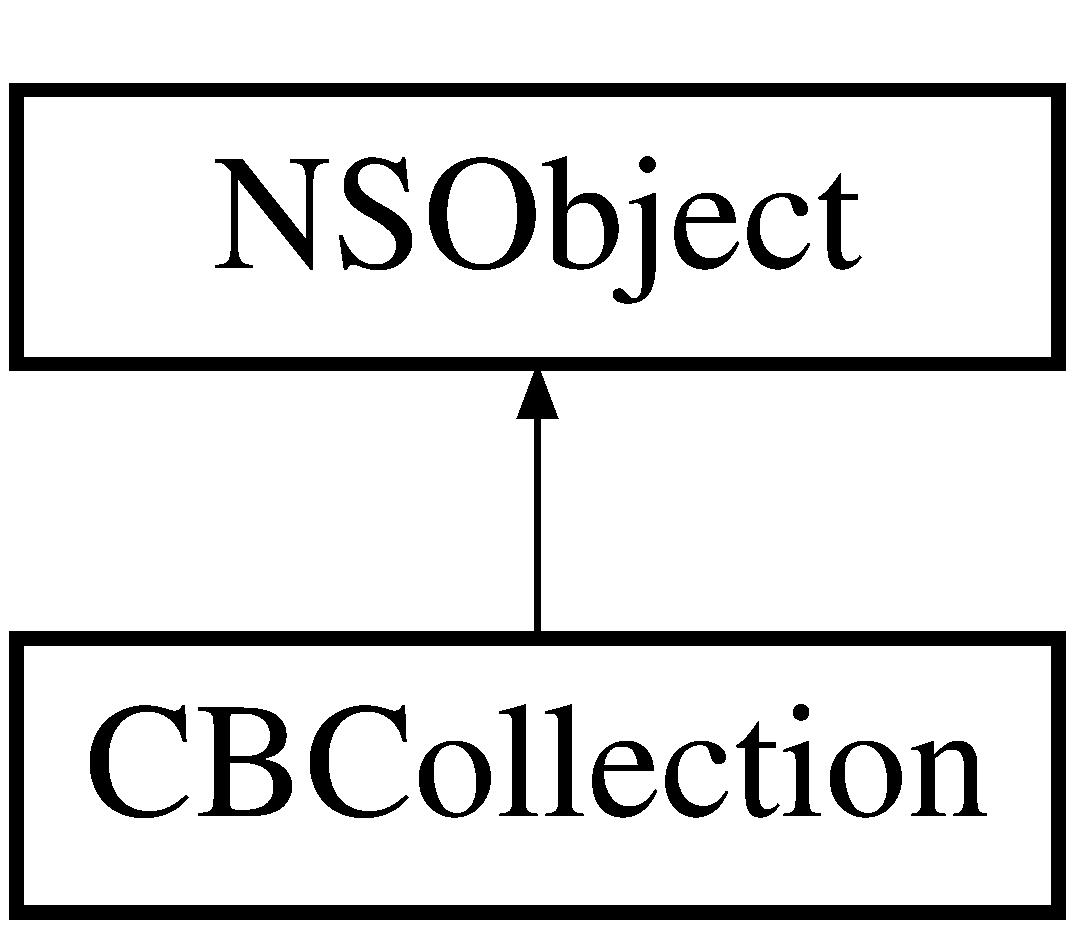
\includegraphics[height=2.000000cm]{interface_c_b_collection}
\end{center}
\end{figure}
\subsection*{Instance Methods}
\begin{DoxyCompactItemize}
\item 
(id) -\/ \hyperlink{interface_c_b_collection_ad232890eefe5c505991479ac6f018f9a}{init\+With\+Collection\+I\+D\+:}
\item 
(void) -\/ \hyperlink{interface_c_b_collection_aebbdb37306fcfa13bcdc915c96c37297}{fetch\+With\+Success\+Callback\+:with\+Error\+Callback\+:}
\item 
(void) -\/ \hyperlink{interface_c_b_collection_ad0e9afe7d01f2bf95510b1e462d31f2d}{fetch\+With\+Query\+:with\+Success\+Callback\+:with\+Error\+Callback\+:}
\item 
(void) -\/ \hyperlink{interface_c_b_collection_a72a5135772c9829d253fb614887158b4}{create\+With\+Data\+:with\+Success\+Callback\+:with\+Error\+Callback\+:}
\item 
(void) -\/ \hyperlink{interface_c_b_collection_af556b08ec3e81638b50b0bc8e06a9938}{update\+With\+Query\+:with\+Changes\+:with\+Success\+Callback\+:with\+Error\+Callback\+:}
\item 
(void) -\/ \hyperlink{interface_c_b_collection_a020a60192df9f85305aea894a19ac9ec}{remove\+With\+Query\+:with\+Success\+Callback\+:with\+Error\+Callback\+:}
\end{DoxyCompactItemize}
\subsection*{Class Methods}
\begin{DoxyCompactItemize}
\item 
(\hyperlink{interface_c_b_collection}{C\+B\+Collection} $\ast$) + \hyperlink{interface_c_b_collection_ad0d5e667992df0fbeedc094edd29375b}{collection\+With\+I\+D\+:}
\end{DoxyCompactItemize}
\subsection*{Properties}
\begin{DoxyCompactItemize}
\item 
N\+S\+String $\ast$ \hyperlink{interface_c_b_collection_a526d5990ac9db1922300bc55bc764fc1}{collection\+I\+D}
\end{DoxyCompactItemize}


\subsection{Detailed Description}
Class for dealing with \hyperlink{interface_clear_blade}{Clear\+Blade} Platform Collections. 

\subsection{Method Documentation}
\hypertarget{interface_c_b_collection_ad0d5e667992df0fbeedc094edd29375b}{\index{C\+B\+Collection@{C\+B\+Collection}!collection\+With\+I\+D\+:@{collection\+With\+I\+D\+:}}
\index{collection\+With\+I\+D\+:@{collection\+With\+I\+D\+:}!CBCollection@{C\+B\+Collection}}
\subsubsection[{collection\+With\+I\+D\+:}]{\setlength{\rightskip}{0pt plus 5cm}+ ({\bf C\+B\+Collection} $\ast$) collection\+With\+I\+D\+: 
\begin{DoxyParamCaption}
\item[{(N\+S\+String $\ast$)}]{collection\+I\+D}
\end{DoxyParamCaption}
}}\label{interface_c_b_collection_ad0d5e667992df0fbeedc094edd29375b}
Initialize a new \hyperlink{interface_c_b_collection}{C\+B\+Collection} object 
\begin{DoxyParams}{Parameters}
{\em collection\+I\+D} & The string that will be used to identify the collection on the server \\
\hline
\end{DoxyParams}
\begin{DoxyReturn}{Returns}
a newly initialized object 
\end{DoxyReturn}
\hypertarget{interface_c_b_collection_a72a5135772c9829d253fb614887158b4}{\index{C\+B\+Collection@{C\+B\+Collection}!create\+With\+Data\+:with\+Success\+Callback\+:with\+Error\+Callback\+:@{create\+With\+Data\+:with\+Success\+Callback\+:with\+Error\+Callback\+:}}
\index{create\+With\+Data\+:with\+Success\+Callback\+:with\+Error\+Callback\+:@{create\+With\+Data\+:with\+Success\+Callback\+:with\+Error\+Callback\+:}!CBCollection@{C\+B\+Collection}}
\subsubsection[{create\+With\+Data\+:with\+Success\+Callback\+:with\+Error\+Callback\+:}]{\setlength{\rightskip}{0pt plus 5cm}-\/ (void) create\+With\+Data\+: 
\begin{DoxyParamCaption}
\item[{(N\+S\+Dictionary $\ast$)}]{data}
\item[{withSuccessCallback:(C\+B\+Item\+Success\+Callback)}]{success\+Callback}
\item[{withErrorCallback:(C\+B\+Item\+Error\+Callback)}]{failure\+Callback}
\end{DoxyParamCaption}
}}\label{interface_c_b_collection_a72a5135772c9829d253fb614887158b4}
Creates a new Item in the collection in the Platform. This creates a new item on the server. 
\begin{DoxyParams}{Parameters}
{\em data} & A Dictionary that contains the object that you want the item in the platform to represent \\
\hline
{\em success\+Callback} & Callback Block to handle successfully returned data \\
\hline
{\em failure\+Callback} & Callback Block to handle errors returned \\
\hline
\end{DoxyParams}
\hypertarget{interface_c_b_collection_ad0e9afe7d01f2bf95510b1e462d31f2d}{\index{C\+B\+Collection@{C\+B\+Collection}!fetch\+With\+Query\+:with\+Success\+Callback\+:with\+Error\+Callback\+:@{fetch\+With\+Query\+:with\+Success\+Callback\+:with\+Error\+Callback\+:}}
\index{fetch\+With\+Query\+:with\+Success\+Callback\+:with\+Error\+Callback\+:@{fetch\+With\+Query\+:with\+Success\+Callback\+:with\+Error\+Callback\+:}!CBCollection@{C\+B\+Collection}}
\subsubsection[{fetch\+With\+Query\+:with\+Success\+Callback\+:with\+Error\+Callback\+:}]{\setlength{\rightskip}{0pt plus 5cm}-\/ (void) fetch\+With\+Query\+: 
\begin{DoxyParamCaption}
\item[{({\bf C\+B\+Query}$\ast$)}]{query}
\item[{withSuccessCallback:(C\+B\+Query\+Success\+Callback)}]{success\+Callback}
\item[{withErrorCallback:(C\+B\+Query\+Error\+Callback)}]{failure\+Callback}
\end{DoxyParamCaption}
}}\label{interface_c_b_collection_ad0e9afe7d01f2bf95510b1e462d31f2d}
Fetches all data from the collection that matches a particular query 
\begin{DoxyParams}{Parameters}
{\em query} & A \hyperlink{interface_c_b_query}{C\+B\+Query} object that defines what you want returned from the Platform \\
\hline
{\em success\+Callback} & Callback Block to handle successfully returned data \\
\hline
{\em failure\+Callback} & Callback Block to handle errors returned \\
\hline
\end{DoxyParams}
\hypertarget{interface_c_b_collection_aebbdb37306fcfa13bcdc915c96c37297}{\index{C\+B\+Collection@{C\+B\+Collection}!fetch\+With\+Success\+Callback\+:with\+Error\+Callback\+:@{fetch\+With\+Success\+Callback\+:with\+Error\+Callback\+:}}
\index{fetch\+With\+Success\+Callback\+:with\+Error\+Callback\+:@{fetch\+With\+Success\+Callback\+:with\+Error\+Callback\+:}!CBCollection@{C\+B\+Collection}}
\subsubsection[{fetch\+With\+Success\+Callback\+:with\+Error\+Callback\+:}]{\setlength{\rightskip}{0pt plus 5cm}-\/ (void) fetch\+With\+Success\+Callback\+: 
\begin{DoxyParamCaption}
\item[{(C\+B\+Query\+Success\+Callback)}]{success\+Callback}
\item[{withErrorCallback:(C\+B\+Query\+Error\+Callback)}]{failure\+Callback}
\end{DoxyParamCaption}
}}\label{interface_c_b_collection_aebbdb37306fcfa13bcdc915c96c37297}
Fetches the entire collection from the Platform. The returned data will be returned to the block you provide 
\begin{DoxyParams}{Parameters}
{\em success\+Callback} & Callback Block to handle successfully returned data \\
\hline
{\em failure\+Callback} & Callback Block to handle errors returned \\
\hline
\end{DoxyParams}
\hypertarget{interface_c_b_collection_ad232890eefe5c505991479ac6f018f9a}{\index{C\+B\+Collection@{C\+B\+Collection}!init\+With\+Collection\+I\+D\+:@{init\+With\+Collection\+I\+D\+:}}
\index{init\+With\+Collection\+I\+D\+:@{init\+With\+Collection\+I\+D\+:}!CBCollection@{C\+B\+Collection}}
\subsubsection[{init\+With\+Collection\+I\+D\+:}]{\setlength{\rightskip}{0pt plus 5cm}-\/ (id) init\+With\+Collection\+I\+D\+: 
\begin{DoxyParamCaption}
\item[{(N\+S\+String $\ast$)}]{col\+I\+D}
\end{DoxyParamCaption}
}}\label{interface_c_b_collection_ad232890eefe5c505991479ac6f018f9a}
Initialize a new \hyperlink{interface_c_b_collection}{C\+B\+Collection} object 
\begin{DoxyParams}{Parameters}
{\em col\+I\+D} & The string that will be used to identify the collection on the server \\
\hline
\end{DoxyParams}
\begin{DoxyReturn}{Returns}
a newly initialized object 
\end{DoxyReturn}
\hypertarget{interface_c_b_collection_a020a60192df9f85305aea894a19ac9ec}{\index{C\+B\+Collection@{C\+B\+Collection}!remove\+With\+Query\+:with\+Success\+Callback\+:with\+Error\+Callback\+:@{remove\+With\+Query\+:with\+Success\+Callback\+:with\+Error\+Callback\+:}}
\index{remove\+With\+Query\+:with\+Success\+Callback\+:with\+Error\+Callback\+:@{remove\+With\+Query\+:with\+Success\+Callback\+:with\+Error\+Callback\+:}!CBCollection@{C\+B\+Collection}}
\subsubsection[{remove\+With\+Query\+:with\+Success\+Callback\+:with\+Error\+Callback\+:}]{\setlength{\rightskip}{0pt plus 5cm}-\/ (void) remove\+With\+Query\+: 
\begin{DoxyParamCaption}
\item[{({\bf C\+B\+Query} $\ast$)}]{query}
\item[{withSuccessCallback:(C\+B\+Query\+Success\+Callback)}]{success\+Callback}
\item[{withErrorCallback:(C\+B\+Query\+Error\+Callback)}]{failure\+Callback}
\end{DoxyParamCaption}
}}\label{interface_c_b_collection_a020a60192df9f85305aea894a19ac9ec}
Removes an item or a set of items on the Platform that match the given query. 
\begin{DoxyParams}{Parameters}
{\em query} & A \hyperlink{interface_c_b_query}{C\+B\+Query} object that defines what you want removed from the Platform \\
\hline
{\em success\+Callback} & Callback Block to handle successfully returned data \\
\hline
{\em failure\+Callback} & Callback Block to handle errors returned \\
\hline
\end{DoxyParams}
\hypertarget{interface_c_b_collection_af556b08ec3e81638b50b0bc8e06a9938}{\index{C\+B\+Collection@{C\+B\+Collection}!update\+With\+Query\+:with\+Changes\+:with\+Success\+Callback\+:with\+Error\+Callback\+:@{update\+With\+Query\+:with\+Changes\+:with\+Success\+Callback\+:with\+Error\+Callback\+:}}
\index{update\+With\+Query\+:with\+Changes\+:with\+Success\+Callback\+:with\+Error\+Callback\+:@{update\+With\+Query\+:with\+Changes\+:with\+Success\+Callback\+:with\+Error\+Callback\+:}!CBCollection@{C\+B\+Collection}}
\subsubsection[{update\+With\+Query\+:with\+Changes\+:with\+Success\+Callback\+:with\+Error\+Callback\+:}]{\setlength{\rightskip}{0pt plus 5cm}-\/ (void) update\+With\+Query\+: 
\begin{DoxyParamCaption}
\item[{({\bf C\+B\+Query} $\ast$)}]{query}
\item[{withChanges:(N\+S\+Dictionary $\ast$)}]{changes}
\item[{withSuccessCallback:(C\+B\+Query\+Success\+Callback)}]{success\+Callback}
\item[{withErrorCallback:(C\+B\+Query\+Error\+Callback)}]{failure\+Callback}
\end{DoxyParamCaption}
}}\label{interface_c_b_collection_af556b08ec3e81638b50b0bc8e06a9938}
Updates an item or a set of items on the Platform that match the given query. 
\begin{DoxyParams}{Parameters}
{\em query} & A \hyperlink{interface_c_b_query}{C\+B\+Query} object that defines what you want updated on the Platform \\
\hline
{\em changes} & A Dictionary containing all of the changes that you want to make on items that match the query. \\
\hline
{\em success\+Callback} & Callback Block to handle successfully returned data \\
\hline
{\em failure\+Callback} & Callback Block to handle errors returned \\
\hline
\end{DoxyParams}


\subsection{Property Documentation}
\hypertarget{interface_c_b_collection_a526d5990ac9db1922300bc55bc764fc1}{\index{C\+B\+Collection@{C\+B\+Collection}!collection\+I\+D@{collection\+I\+D}}
\index{collection\+I\+D@{collection\+I\+D}!CBCollection@{C\+B\+Collection}}
\subsubsection[{collection\+I\+D}]{\setlength{\rightskip}{0pt plus 5cm}-\/ (N\+S\+String$\ast$) collection\+I\+D\hspace{0.3cm}{\ttfamily [read]}, {\ttfamily [write]}, {\ttfamily [nonatomic]}, {\ttfamily [strong]}}}\label{interface_c_b_collection_a526d5990ac9db1922300bc55bc764fc1}
The string that represents the collection I\+D. 

The documentation for this class was generated from the following files\+:\begin{DoxyCompactItemize}
\item 
C\+B\+Collection.\+h\item 
C\+B\+Collection.\+m\end{DoxyCompactItemize}

\hypertarget{interface_c_b_h_t_t_p_request}{\section{C\+B\+H\+T\+T\+P\+Request Class Reference}
\label{interface_c_b_h_t_t_p_request}\index{C\+B\+H\+T\+T\+P\+Request@{C\+B\+H\+T\+T\+P\+Request}}
}
Inheritance diagram for C\+B\+H\+T\+T\+P\+Request\+:\begin{figure}[H]
\begin{center}
\leavevmode
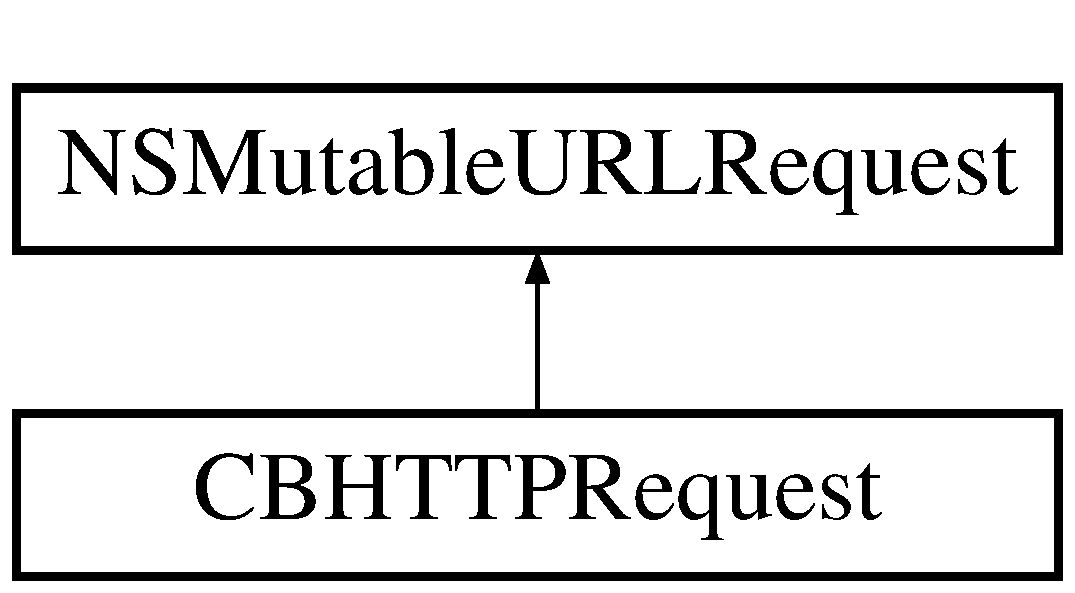
\includegraphics[height=2.000000cm]{interface_c_b_h_t_t_p_request}
\end{center}
\end{figure}
\subsection*{Instance Methods}
\begin{DoxyCompactItemize}
\item 
\hypertarget{interface_c_b_h_t_t_p_request_a2053e38ef61e8235127755881330f944}{(instancetype) -\/ {\bfseries init\+With\+Clear\+Blade\+Settings\+:with\+Method\+:with\+Collection\+:with\+Parameters\+:with\+User\+:}}\label{interface_c_b_h_t_t_p_request_a2053e38ef61e8235127755881330f944}

\item 
\hypertarget{interface_c_b_h_t_t_p_request_a69d8aa14a2fd7ac624c1a2a220a426b9}{(N\+S\+Data $\ast$) -\/ {\bfseries execute\+With\+Error\+:}}\label{interface_c_b_h_t_t_p_request_a69d8aa14a2fd7ac624c1a2a220a426b9}

\item 
\hypertarget{interface_c_b_h_t_t_p_request_ad5c510894450d80dc40f9ff0d23df048}{(void) -\/ {\bfseries execute\+With\+Success\+Callback\+:with\+Error\+Callback\+:}}\label{interface_c_b_h_t_t_p_request_ad5c510894450d80dc40f9ff0d23df048}

\end{DoxyCompactItemize}
\subsection*{Class Methods}
\begin{DoxyCompactItemize}
\item 
\hypertarget{interface_c_b_h_t_t_p_request_acb09f64190f8a279405d1fa1bc62bb6d}{(instancetype) + {\bfseries request\+With\+Method\+:with\+Collection\+:with\+Parameters\+:with\+User\+:}}\label{interface_c_b_h_t_t_p_request_acb09f64190f8a279405d1fa1bc62bb6d}

\item 
\hypertarget{interface_c_b_h_t_t_p_request_a6e8528264293eccf7256128a2e46dff2}{(instancetype) + {\bfseries user\+Request\+With\+Settings\+:with\+Method\+:with\+Action\+:with\+Body\+:with\+Headers\+:}}\label{interface_c_b_h_t_t_p_request_a6e8528264293eccf7256128a2e46dff2}

\end{DoxyCompactItemize}
\subsection*{Properties}
\begin{DoxyCompactItemize}
\item 
\hypertarget{interface_c_b_h_t_t_p_request_a7724199e4703f73b856f2ec2262e5735}{\hyperlink{interface_clear_blade}{Clear\+Blade} $\ast$ {\bfseries settings}}\label{interface_c_b_h_t_t_p_request_a7724199e4703f73b856f2ec2262e5735}

\item 
\hypertarget{interface_c_b_h_t_t_p_request_a8da1f5fa0eef6eef45d22eb694ae3039}{\hyperlink{interface_c_b_user}{C\+B\+User} $\ast$ {\bfseries user}}\label{interface_c_b_h_t_t_p_request_a8da1f5fa0eef6eef45d22eb694ae3039}

\item 
\hypertarget{interface_c_b_h_t_t_p_request_ad37d5f489778cda66ace537ee166cd8e}{N\+S\+String $\ast$ {\bfseries action}}\label{interface_c_b_h_t_t_p_request_ad37d5f489778cda66ace537ee166cd8e}

\end{DoxyCompactItemize}


The documentation for this class was generated from the following files\+:\begin{DoxyCompactItemize}
\item 
Clear\+Blade\+A\+P\+I/C\+B\+H\+T\+T\+P\+Request.\+h\item 
Clear\+Blade\+A\+P\+I/C\+B\+H\+T\+T\+P\+Request.\+m\end{DoxyCompactItemize}

\hypertarget{interface_c_b_h_t_t_p_request_response}{\section{C\+B\+H\+T\+T\+P\+Request\+Response Class Reference}
\label{interface_c_b_h_t_t_p_request_response}\index{C\+B\+H\+T\+T\+P\+Request\+Response@{C\+B\+H\+T\+T\+P\+Request\+Response}}
}
Inheritance diagram for C\+B\+H\+T\+T\+P\+Request\+Response\+:\begin{figure}[H]
\begin{center}
\leavevmode
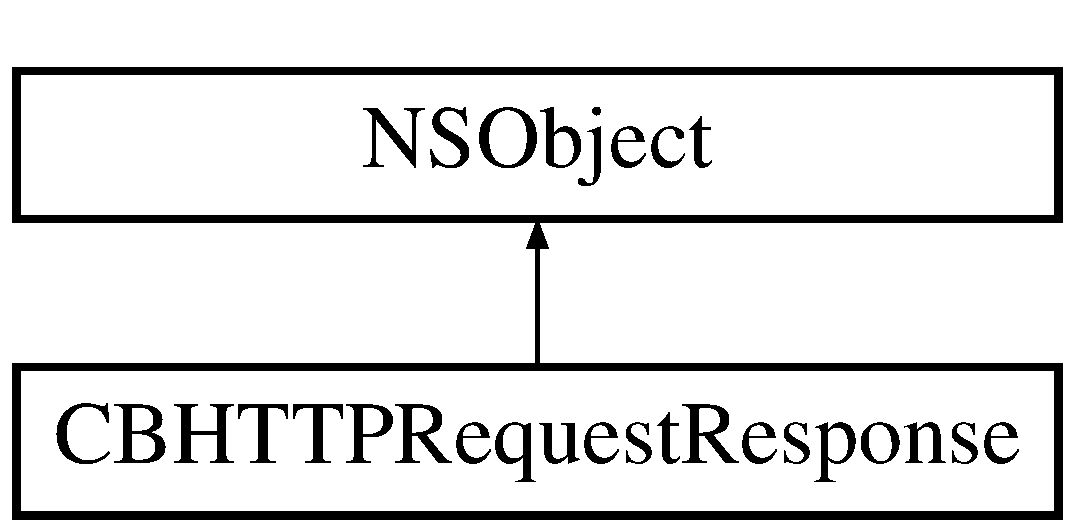
\includegraphics[height=2.000000cm]{interface_c_b_h_t_t_p_request_response}
\end{center}
\end{figure}
\subsection*{Class Methods}
\begin{DoxyCompactItemize}
\item 
\hypertarget{interface_c_b_h_t_t_p_request_response_adf76e986c5ec2fb394c27f23331fb680}{(instancetype) + {\bfseries response\+With\+Request\+:with\+Response\+:with\+Data\+:}}\label{interface_c_b_h_t_t_p_request_response_adf76e986c5ec2fb394c27f23331fb680}

\end{DoxyCompactItemize}
\subsection*{Properties}
\begin{DoxyCompactItemize}
\item 
\hypertarget{interface_c_b_h_t_t_p_request_response_a47ccbfe884900d45f4f8e0a0b4fafea7}{\hyperlink{interface_c_b_h_t_t_p_request}{C\+B\+H\+T\+T\+P\+Request} $\ast$ {\bfseries request}}\label{interface_c_b_h_t_t_p_request_response_a47ccbfe884900d45f4f8e0a0b4fafea7}

\item 
\hypertarget{interface_c_b_h_t_t_p_request_response_adf582af8f5400ad6fbe784b87e1b2eaf}{N\+S\+H\+T\+T\+P\+U\+R\+L\+Response $\ast$ {\bfseries response}}\label{interface_c_b_h_t_t_p_request_response_adf582af8f5400ad6fbe784b87e1b2eaf}

\item 
\hypertarget{interface_c_b_h_t_t_p_request_response_a1006216c5a63489696bffc15fffba1b3}{N\+S\+Data $\ast$ {\bfseries response\+Data}}\label{interface_c_b_h_t_t_p_request_response_a1006216c5a63489696bffc15fffba1b3}

\item 
\hypertarget{interface_c_b_h_t_t_p_request_response_ac90c310149a1720766bcbe8f0d2e429d}{N\+S\+String $\ast$ {\bfseries response\+String}}\label{interface_c_b_h_t_t_p_request_response_ac90c310149a1720766bcbe8f0d2e429d}

\end{DoxyCompactItemize}


The documentation for this class was generated from the following files\+:\begin{DoxyCompactItemize}
\item 
Clear\+Blade\+A\+P\+I/C\+B\+H\+T\+T\+P\+Request\+Response.\+h\item 
Clear\+Blade\+A\+P\+I/C\+B\+H\+T\+T\+P\+Request\+Response.\+m\end{DoxyCompactItemize}

\hypertarget{interface_c_b_item}{\section{C\+B\+Item Class Reference}
\label{interface_c_b_item}\index{C\+B\+Item@{C\+B\+Item}}
}


{\ttfamily \#import $<$C\+B\+Item.\+h$>$}

Inheritance diagram for C\+B\+Item\+:\begin{figure}[H]
\begin{center}
\leavevmode
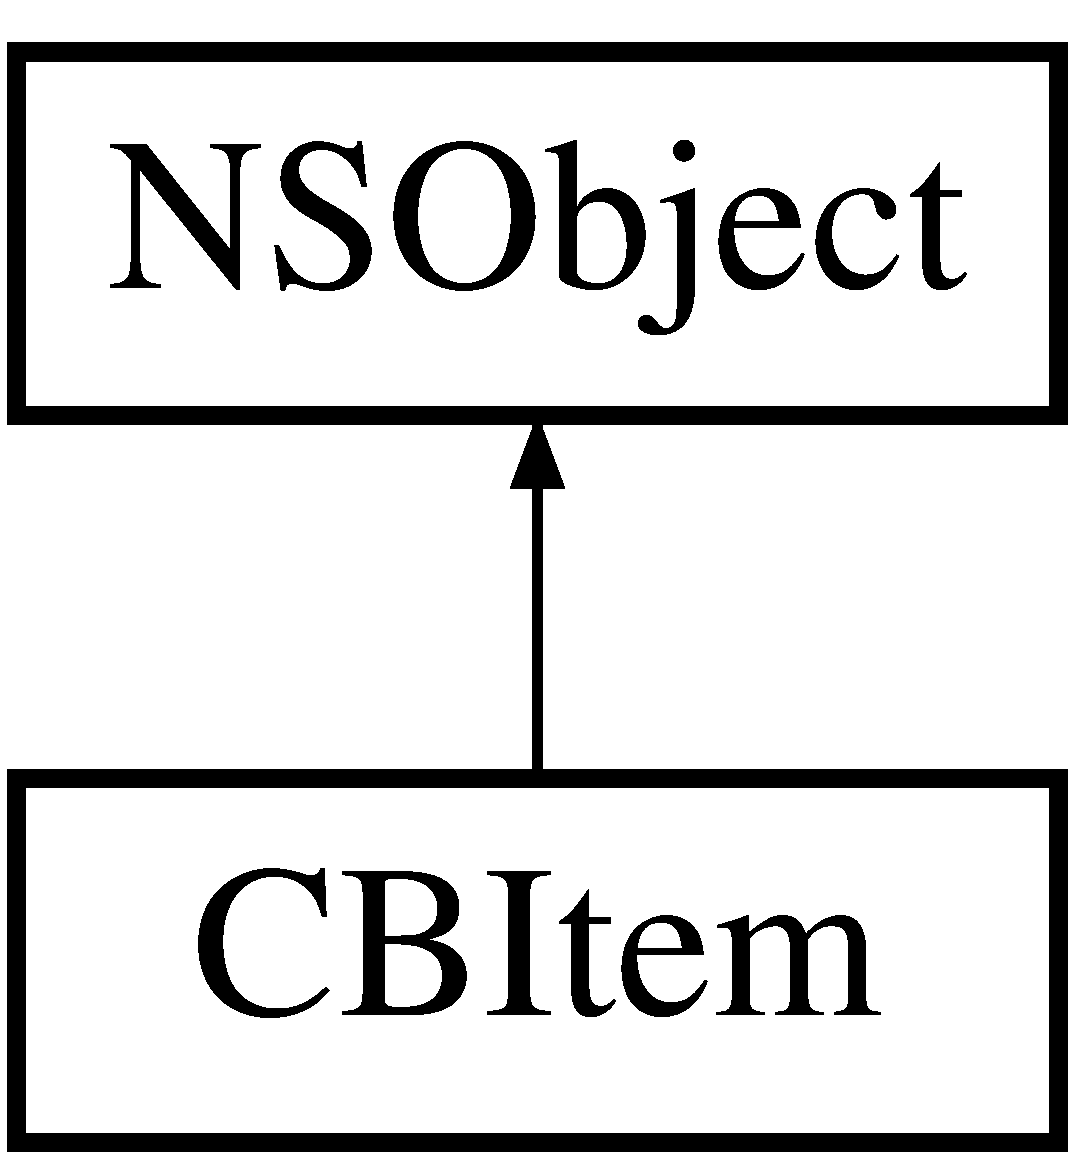
\includegraphics[height=2.000000cm]{interface_c_b_item}
\end{center}
\end{figure}
\subsection*{Instance Methods}
\begin{DoxyCompactItemize}
\item 
(instancetype) -\/ \hyperlink{interface_c_b_item_ace72b56932f3aa3b636800abdb50daa0}{init\+With\+Data\+:with\+Collection\+I\+D\+:}
\item 
(void) -\/ \hyperlink{interface_c_b_item_a35bde628ed02786ebcd145d74bea5ead}{save\+With\+Success\+Callback\+:with\+Error\+Callback\+:}
\item 
(void) -\/ \hyperlink{interface_c_b_item_acb4af198992cddea658fb099bbd81583}{refresh\+With\+Success\+Callback\+:with\+Error\+Callback\+:}
\item 
(void) -\/ \hyperlink{interface_c_b_item_acc375a79b97c2fcfaeda1c2737de51c0}{remove\+With\+Success\+Callback\+:with\+Error\+Callback\+:}
\item 
(id) -\/ \hyperlink{interface_c_b_item_aeb280c9120217ef525b1c47adb5db344}{object\+For\+Key\+:}
\item 
\hypertarget{interface_c_b_item_a850d0c9f26e8cd83ddec83458bc57df8}{(void) -\/ {\bfseries set\+Object\+:for\+Key\+:}}\label{interface_c_b_item_a850d0c9f26e8cd83ddec83458bc57df8}

\item 
(bool) -\/ \hyperlink{interface_c_b_item_ab47361f0044a8fd1893823b6ec95c46f}{is\+Equal\+To\+C\+B\+Item\+:}
\end{DoxyCompactItemize}
\subsection*{Class Methods}
\begin{DoxyCompactItemize}
\item 
(instancetype) + \hyperlink{interface_c_b_item_a5f9b22377c54afcb79916eaa66108140}{item\+With\+Data\+:with\+Collection\+I\+D\+:}
\item 
\hypertarget{interface_c_b_item_ab370a3dfb1ce240b8c59b41436532e56}{(N\+S\+Mutable\+Array $\ast$) + {\bfseries array\+Of\+C\+B\+Items\+From\+Array\+Of\+Dictionaries\+:with\+Collection\+I\+D\+:}}\label{interface_c_b_item_ab370a3dfb1ce240b8c59b41436532e56}

\end{DoxyCompactItemize}
\subsection*{Properties}
\begin{DoxyCompactItemize}
\item 
N\+S\+Mutable\+Dictionary $\ast$ \hyperlink{interface_c_b_item_a056a3d35cb718cb306dc69915bec29e2}{data}
\item 
N\+S\+String $\ast$ \hyperlink{interface_c_b_item_a8d47dba1bcfeb0754b65d312a48a939a}{collection\+I\+D}
\item 
N\+S\+String $\ast$ \hyperlink{interface_c_b_item_adc7d0932fa46e75354e7dbe63d714165}{item\+I\+D}
\end{DoxyCompactItemize}


\subsection{Detailed Description}
Class that represents an individual item from the platform 

\subsection{Method Documentation}
\hypertarget{interface_c_b_item_ace72b56932f3aa3b636800abdb50daa0}{\index{C\+B\+Item@{C\+B\+Item}!init\+With\+Data\+:with\+Collection\+I\+D\+:@{init\+With\+Data\+:with\+Collection\+I\+D\+:}}
\index{init\+With\+Data\+:with\+Collection\+I\+D\+:@{init\+With\+Data\+:with\+Collection\+I\+D\+:}!C\+B\+Item@{C\+B\+Item}}
\subsubsection[{init\+With\+Data\+:with\+Collection\+I\+D\+:}]{\setlength{\rightskip}{0pt plus 5cm}-\/ (instancetype) init\+With\+Data\+: 
\begin{DoxyParamCaption}
\item[{(N\+S\+Dictionary $\ast$)}]{input\+Data}
\item[{withCollectionID:(N\+S\+String $\ast$)}]{col\+I\+D}
\end{DoxyParamCaption}
}}\label{interface_c_b_item_ace72b56932f3aa3b636800abdb50daa0}
Initializes the Item with data and sets the data and collection\+I\+D. 
\begin{DoxyParams}{Parameters}
{\em input\+Data} & A dictionary that holds data for the item \\
\hline
{\em col\+I\+D} & A string that holds the I\+D of the collection to which this item belongs \\
\hline
\end{DoxyParams}
\begin{DoxyReturn}{Returns}
the newly created \hyperlink{interface_c_b_item}{C\+B\+Item} 
\end{DoxyReturn}
\hypertarget{interface_c_b_item_ab47361f0044a8fd1893823b6ec95c46f}{\index{C\+B\+Item@{C\+B\+Item}!is\+Equal\+To\+C\+B\+Item\+:@{is\+Equal\+To\+C\+B\+Item\+:}}
\index{is\+Equal\+To\+C\+B\+Item\+:@{is\+Equal\+To\+C\+B\+Item\+:}!C\+B\+Item@{C\+B\+Item}}
\subsubsection[{is\+Equal\+To\+C\+B\+Item\+:}]{\setlength{\rightskip}{0pt plus 5cm}-\/ (bool) is\+Equal\+To\+C\+B\+Item\+: 
\begin{DoxyParamCaption}
\item[{({\bf C\+B\+Item} $\ast$)}]{item}
\end{DoxyParamCaption}
}}\label{interface_c_b_item_ab47361f0044a8fd1893823b6ec95c46f}
Checks if all keys on both this \hyperlink{interface_c_b_item}{C\+B\+Item} and the other item are equal. 
\begin{DoxyParams}{Parameters}
{\em item} & The item to check against. \\
\hline
\end{DoxyParams}
\begin{DoxyReturn}{Returns}
true if the other item has all the same keys and values as this item. 
\end{DoxyReturn}
\hypertarget{interface_c_b_item_a5f9b22377c54afcb79916eaa66108140}{\index{C\+B\+Item@{C\+B\+Item}!item\+With\+Data\+:with\+Collection\+I\+D\+:@{item\+With\+Data\+:with\+Collection\+I\+D\+:}}
\index{item\+With\+Data\+:with\+Collection\+I\+D\+:@{item\+With\+Data\+:with\+Collection\+I\+D\+:}!C\+B\+Item@{C\+B\+Item}}
\subsubsection[{item\+With\+Data\+:with\+Collection\+I\+D\+:}]{\setlength{\rightskip}{0pt plus 5cm}+ ({\bf C\+B\+Item} $\ast$) item\+With\+Data\+: 
\begin{DoxyParamCaption}
\item[{(N\+S\+Dictionary $\ast$)}]{input\+Data}
\item[{withCollectionID:(N\+S\+String $\ast$)}]{collection\+I\+D}
\end{DoxyParamCaption}
}}\label{interface_c_b_item_a5f9b22377c54afcb79916eaa66108140}
Creates an Item with data belonging to the collection with collection\+I\+D 
\begin{DoxyParams}{Parameters}
{\em input\+Data} & A dictionary that holds data for the item \\
\hline
{\em collection\+I\+D} & The I\+D of the collection this item will belong to \\
\hline
\end{DoxyParams}
\begin{DoxyReturn}{Returns}
The newly created \hyperlink{interface_c_b_item}{C\+B\+Item} 
\end{DoxyReturn}
\hypertarget{interface_c_b_item_aeb280c9120217ef525b1c47adb5db344}{\index{C\+B\+Item@{C\+B\+Item}!object\+For\+Key\+:@{object\+For\+Key\+:}}
\index{object\+For\+Key\+:@{object\+For\+Key\+:}!C\+B\+Item@{C\+B\+Item}}
\subsubsection[{object\+For\+Key\+:}]{\setlength{\rightskip}{0pt plus 5cm}-\/ (id) object\+For\+Key\+: 
\begin{DoxyParamCaption}
\item[{(N\+S\+String $\ast$)}]{key}
\end{DoxyParamCaption}
}}\label{interface_c_b_item_aeb280c9120217ef525b1c47adb5db344}
Gets an item out of the data attribute that matches the given string 
\begin{DoxyParams}{Parameters}
{\em key} & String used to find a value in the dictionary \\
\hline
\end{DoxyParams}
\begin{DoxyReturn}{Returns}
The id that is referenced by the value for the given key 
\end{DoxyReturn}
\hypertarget{interface_c_b_item_acb4af198992cddea658fb099bbd81583}{\index{C\+B\+Item@{C\+B\+Item}!refresh\+With\+Success\+Callback\+:with\+Error\+Callback\+:@{refresh\+With\+Success\+Callback\+:with\+Error\+Callback\+:}}
\index{refresh\+With\+Success\+Callback\+:with\+Error\+Callback\+:@{refresh\+With\+Success\+Callback\+:with\+Error\+Callback\+:}!C\+B\+Item@{C\+B\+Item}}
\subsubsection[{refresh\+With\+Success\+Callback\+:with\+Error\+Callback\+:}]{\setlength{\rightskip}{0pt plus 5cm}-\/ (void) refresh\+With\+Success\+Callback\+: 
\begin{DoxyParamCaption}
\item[{(C\+B\+Item\+Success\+Callback)}]{success\+Callback}
\item[{withErrorCallback:(C\+B\+Item\+Error\+Callback)}]{error\+Callback}
\end{DoxyParamCaption}
}}\label{interface_c_b_item_acb4af198992cddea658fb099bbd81583}
Pulls down any changes that have been made on the server to the item since being instantiated. This updates the data attribute to reflect the current state of the Item on the server \hypertarget{interface_c_b_item_acc375a79b97c2fcfaeda1c2737de51c0}{\index{C\+B\+Item@{C\+B\+Item}!remove\+With\+Success\+Callback\+:with\+Error\+Callback\+:@{remove\+With\+Success\+Callback\+:with\+Error\+Callback\+:}}
\index{remove\+With\+Success\+Callback\+:with\+Error\+Callback\+:@{remove\+With\+Success\+Callback\+:with\+Error\+Callback\+:}!C\+B\+Item@{C\+B\+Item}}
\subsubsection[{remove\+With\+Success\+Callback\+:with\+Error\+Callback\+:}]{\setlength{\rightskip}{0pt plus 5cm}-\/ (void) remove\+With\+Success\+Callback\+: 
\begin{DoxyParamCaption}
\item[{(C\+B\+Item\+Success\+Callback)}]{success\+Callback}
\item[{withErrorCallback:(C\+B\+Item\+Error\+Callback)}]{error\+Callback}
\end{DoxyParamCaption}
}}\label{interface_c_b_item_acc375a79b97c2fcfaeda1c2737de51c0}
Deletes the Item on the server This cannot be undone. \hypertarget{interface_c_b_item_a35bde628ed02786ebcd145d74bea5ead}{\index{C\+B\+Item@{C\+B\+Item}!save\+With\+Success\+Callback\+:with\+Error\+Callback\+:@{save\+With\+Success\+Callback\+:with\+Error\+Callback\+:}}
\index{save\+With\+Success\+Callback\+:with\+Error\+Callback\+:@{save\+With\+Success\+Callback\+:with\+Error\+Callback\+:}!C\+B\+Item@{C\+B\+Item}}
\subsubsection[{save\+With\+Success\+Callback\+:with\+Error\+Callback\+:}]{\setlength{\rightskip}{0pt plus 5cm}-\/ (void) save\+With\+Success\+Callback\+: 
\begin{DoxyParamCaption}
\item[{(C\+B\+Item\+Success\+Callback)}]{success\+Callback}
\item[{withErrorCallback:(C\+B\+Item\+Error\+Callback)}]{error\+Callback}
\end{DoxyParamCaption}
}}\label{interface_c_b_item_a35bde628ed02786ebcd145d74bea5ead}
Saves any changes that have been made to the data property to the Platform This will update the server 

\subsection{Property Documentation}
\hypertarget{interface_c_b_item_a8d47dba1bcfeb0754b65d312a48a939a}{\index{C\+B\+Item@{C\+B\+Item}!collection\+I\+D@{collection\+I\+D}}
\index{collection\+I\+D@{collection\+I\+D}!C\+B\+Item@{C\+B\+Item}}
\subsubsection[{collection\+I\+D}]{\setlength{\rightskip}{0pt plus 5cm}-\/ (N\+S\+String$\ast$) collection\+I\+D\hspace{0.3cm}{\ttfamily [read]}, {\ttfamily [write]}, {\ttfamily [nonatomic]}, {\ttfamily [strong]}}}\label{interface_c_b_item_a8d47dba1bcfeb0754b65d312a48a939a}
A string holding the I\+D of the collection to which this item belongs \hypertarget{interface_c_b_item_a056a3d35cb718cb306dc69915bec29e2}{\index{C\+B\+Item@{C\+B\+Item}!data@{data}}
\index{data@{data}!C\+B\+Item@{C\+B\+Item}}
\subsubsection[{data}]{\setlength{\rightskip}{0pt plus 5cm}-\/ (N\+S\+Mutable\+Dictionary $\ast$) data\hspace{0.3cm}{\ttfamily [read]}, {\ttfamily [write]}, {\ttfamily [nonatomic]}, {\ttfamily [strong]}}}\label{interface_c_b_item_a056a3d35cb718cb306dc69915bec29e2}
A dictionary that holds the data that was stored in the platform. \hypertarget{interface_c_b_item_adc7d0932fa46e75354e7dbe63d714165}{\index{C\+B\+Item@{C\+B\+Item}!item\+I\+D@{item\+I\+D}}
\index{item\+I\+D@{item\+I\+D}!C\+B\+Item@{C\+B\+Item}}
\subsubsection[{item\+I\+D}]{\setlength{\rightskip}{0pt plus 5cm}-\/ (N\+S\+String $\ast$) item\+I\+D\hspace{0.3cm}{\ttfamily [read]}, {\ttfamily [write]}, {\ttfamily [nonatomic]}, {\ttfamily [strong]}}}\label{interface_c_b_item_adc7d0932fa46e75354e7dbe63d714165}
A string holding the I\+D of the item 

The documentation for this class was generated from the following files\+:\begin{DoxyCompactItemize}
\item 
Clear\+Blade\+A\+P\+I/C\+B\+Item.\+h\item 
Clear\+Blade\+A\+P\+I/C\+B\+Item.\+m\end{DoxyCompactItemize}

\hypertarget{interface_c_b_message}{\section{C\+B\+Message Class Reference}
\label{interface_c_b_message}\index{C\+B\+Message@{C\+B\+Message}}
}


{\ttfamily \#import $<$C\+B\+Message.\+h$>$}

Inheritance diagram for C\+B\+Message\+:\begin{figure}[H]
\begin{center}
\leavevmode
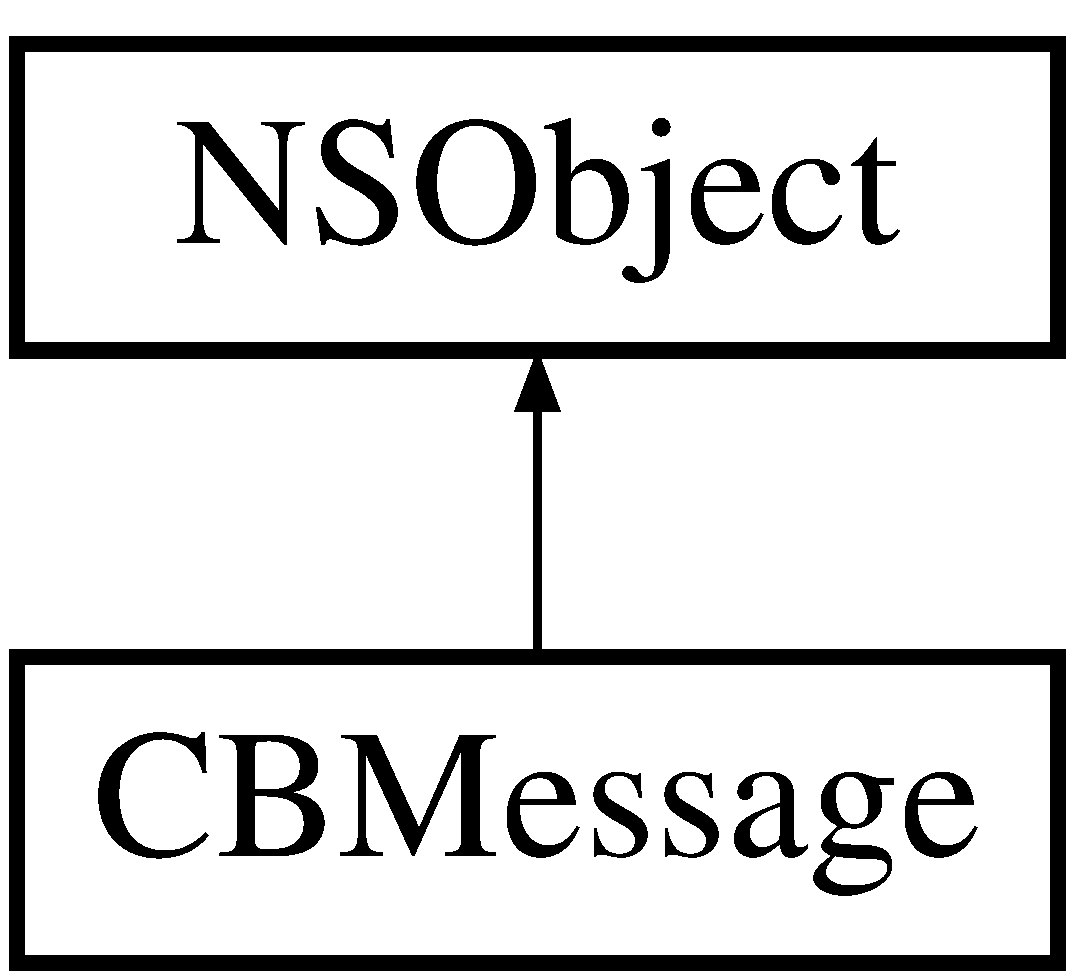
\includegraphics[height=2.000000cm]{interface_c_b_message}
\end{center}
\end{figure}
\subsection*{Instance Methods}
\begin{DoxyCompactItemize}
\item 
(instancetype) -\/ \hyperlink{interface_c_b_message_a38d3e9a65419e27551d38a7628995fb7}{init\+With\+Mosquitto\+Message\+:}
\item 
(instancetype) -\/ \hyperlink{interface_c_b_message_a044bf150504f584117fc5d50f025a26f}{init\+With\+Topic\+:with\+Payload\+Text\+:}
\item 
(instancetype) -\/ \hyperlink{interface_c_b_message_a95a5d53b35af87d89f8fc0c316f0499a}{init\+With\+Topic\+:with\+Payload\+Data\+:}
\end{DoxyCompactItemize}
\subsection*{Class Methods}
\begin{DoxyCompactItemize}
\item 
(instancetype) + \hyperlink{interface_c_b_message_abba382b3f82cd7aebb2f3104ed543602}{message\+With\+Topic\+:with\+Payload\+Text\+:}
\item 
(instancetype) + \hyperlink{interface_c_b_message_a01d6ea86886dec9962ee090d0e76608d}{message\+With\+Topic\+:with\+Payload\+Data\+:}
\item 
(instancetype) + \hyperlink{interface_c_b_message_a3413a6c31ec75df51d2934f5ec58f0db}{message\+From\+Mosquitto\+Message\+:}
\end{DoxyCompactItemize}
\subsection*{Properties}
\begin{DoxyCompactItemize}
\item 
N\+S\+String $\ast$ \hyperlink{interface_c_b_message_a5fef01f2b51495307023ad95e772c632}{topic}
\item 
N\+S\+String $\ast$ \hyperlink{interface_c_b_message_a40254070a83d97673d850d08437fc44b}{payload\+Text}
\item 
N\+S\+Data $\ast$ \hyperlink{interface_c_b_message_a11c9f8c3e5d3e137f6d735ffb3fa7560}{payload\+Data}
\end{DoxyCompactItemize}


\subsection{Detailed Description}
Holds all data for an individual message from M\+Q\+T\+T 

\subsection{Method Documentation}
\hypertarget{interface_c_b_message_a38d3e9a65419e27551d38a7628995fb7}{\index{C\+B\+Message@{C\+B\+Message}!init\+With\+Mosquitto\+Message\+:@{init\+With\+Mosquitto\+Message\+:}}
\index{init\+With\+Mosquitto\+Message\+:@{init\+With\+Mosquitto\+Message\+:}!CBMessage@{C\+B\+Message}}
\subsubsection[{init\+With\+Mosquitto\+Message\+:}]{\setlength{\rightskip}{0pt plus 5cm}-\/ (id) init\+With\+Mosquitto\+Message\+: 
\begin{DoxyParamCaption}
\item[{(const struct mosquitto\+\_\+message $\ast$)}]{message}
\end{DoxyParamCaption}
}}\label{interface_c_b_message_a38d3e9a65419e27551d38a7628995fb7}
Initiates a message using a mosquitto\+\_\+message struct 
\begin{DoxyParams}{Parameters}
{\em message} & The mosquitto\+\_\+message struct used to initialize the \hyperlink{interface_c_b_message}{C\+B\+Message} \\
\hline
\end{DoxyParams}
\begin{DoxyReturn}{Returns}
The initialized \hyperlink{interface_c_b_message}{C\+B\+Message} 
\end{DoxyReturn}
\hypertarget{interface_c_b_message_a95a5d53b35af87d89f8fc0c316f0499a}{\index{C\+B\+Message@{C\+B\+Message}!init\+With\+Topic\+:with\+Payload\+Data\+:@{init\+With\+Topic\+:with\+Payload\+Data\+:}}
\index{init\+With\+Topic\+:with\+Payload\+Data\+:@{init\+With\+Topic\+:with\+Payload\+Data\+:}!CBMessage@{C\+B\+Message}}
\subsubsection[{init\+With\+Topic\+:with\+Payload\+Data\+:}]{\setlength{\rightskip}{0pt plus 5cm}-\/ (instancetype) init\+With\+Topic\+: 
\begin{DoxyParamCaption}
\item[{(N\+S\+String $\ast$)}]{topic}
\item[{withPayloadData:(N\+S\+Data $\ast$)}]{data}
\end{DoxyParamCaption}
}}\label{interface_c_b_message_a95a5d53b35af87d89f8fc0c316f0499a}
Initiates a message using a topic and message data 
\begin{DoxyParams}{Parameters}
{\em topic} & A string with the topic name \\
\hline
{\em data} & A N\+S\+Data object with the payload \\
\hline
\end{DoxyParams}
\begin{DoxyReturn}{Returns}
The created message 
\end{DoxyReturn}
\hypertarget{interface_c_b_message_a044bf150504f584117fc5d50f025a26f}{\index{C\+B\+Message@{C\+B\+Message}!init\+With\+Topic\+:with\+Payload\+Text\+:@{init\+With\+Topic\+:with\+Payload\+Text\+:}}
\index{init\+With\+Topic\+:with\+Payload\+Text\+:@{init\+With\+Topic\+:with\+Payload\+Text\+:}!CBMessage@{C\+B\+Message}}
\subsubsection[{init\+With\+Topic\+:with\+Payload\+Text\+:}]{\setlength{\rightskip}{0pt plus 5cm}-\/ (instancetype) init\+With\+Topic\+: 
\begin{DoxyParamCaption}
\item[{(N\+S\+String $\ast$)}]{topic}
\item[{withPayloadText:(N\+S\+String $\ast$)}]{text}
\end{DoxyParamCaption}
}}\label{interface_c_b_message_a044bf150504f584117fc5d50f025a26f}
Initiates a message using a topic and message string 
\begin{DoxyParams}{Parameters}
{\em topic} & A string with the topic name \\
\hline
{\em text} & A string with the payload text or message \\
\hline
\end{DoxyParams}
\begin{DoxyReturn}{Returns}
The created message 
\end{DoxyReturn}
\hypertarget{interface_c_b_message_a3413a6c31ec75df51d2934f5ec58f0db}{\index{C\+B\+Message@{C\+B\+Message}!message\+From\+Mosquitto\+Message\+:@{message\+From\+Mosquitto\+Message\+:}}
\index{message\+From\+Mosquitto\+Message\+:@{message\+From\+Mosquitto\+Message\+:}!CBMessage@{C\+B\+Message}}
\subsubsection[{message\+From\+Mosquitto\+Message\+:}]{\setlength{\rightskip}{0pt plus 5cm}+ ({\bf C\+B\+Message} $\ast$) message\+From\+Mosquitto\+Message\+: 
\begin{DoxyParamCaption}
\item[{(const struct mosquitto\+\_\+message $\ast$)}]{message}
\end{DoxyParamCaption}
}}\label{interface_c_b_message_a3413a6c31ec75df51d2934f5ec58f0db}
Creates a message from a mosquitto\+\_\+message struct 
\begin{DoxyParams}{Parameters}
{\em message} & The mosquitto\+\_\+message struct to convert from \\
\hline
\end{DoxyParams}
\begin{DoxyReturn}{Returns}
The created message 
\end{DoxyReturn}
\hypertarget{interface_c_b_message_a01d6ea86886dec9962ee090d0e76608d}{\index{C\+B\+Message@{C\+B\+Message}!message\+With\+Topic\+:with\+Payload\+Data\+:@{message\+With\+Topic\+:with\+Payload\+Data\+:}}
\index{message\+With\+Topic\+:with\+Payload\+Data\+:@{message\+With\+Topic\+:with\+Payload\+Data\+:}!CBMessage@{C\+B\+Message}}
\subsubsection[{message\+With\+Topic\+:with\+Payload\+Data\+:}]{\setlength{\rightskip}{0pt plus 5cm}+ (instancetype) message\+With\+Topic\+: 
\begin{DoxyParamCaption}
\item[{(N\+S\+String $\ast$)}]{topic}
\item[{withPayloadData:(N\+S\+Data $\ast$)}]{data}
\end{DoxyParamCaption}
}}\label{interface_c_b_message_a01d6ea86886dec9962ee090d0e76608d}
Creates a message with the given topic and text 
\begin{DoxyParams}{Parameters}
{\em topic} & A string with the topic name \\
\hline
{\em data} & A N\+S\+Data object that represents the payload of the message \\
\hline
\end{DoxyParams}
\begin{DoxyReturn}{Returns}
The created message 
\end{DoxyReturn}
\hypertarget{interface_c_b_message_abba382b3f82cd7aebb2f3104ed543602}{\index{C\+B\+Message@{C\+B\+Message}!message\+With\+Topic\+:with\+Payload\+Text\+:@{message\+With\+Topic\+:with\+Payload\+Text\+:}}
\index{message\+With\+Topic\+:with\+Payload\+Text\+:@{message\+With\+Topic\+:with\+Payload\+Text\+:}!CBMessage@{C\+B\+Message}}
\subsubsection[{message\+With\+Topic\+:with\+Payload\+Text\+:}]{\setlength{\rightskip}{0pt plus 5cm}+ (instancetype) message\+With\+Topic\+: 
\begin{DoxyParamCaption}
\item[{(N\+S\+String $\ast$)}]{topic}
\item[{withPayloadText:(N\+S\+String $\ast$)}]{text}
\end{DoxyParamCaption}
}}\label{interface_c_b_message_abba382b3f82cd7aebb2f3104ed543602}
Creates a message with the given topic and text 
\begin{DoxyParams}{Parameters}
{\em topic} & A string with the topic name \\
\hline
{\em text} & A string with the payload text or message \\
\hline
\end{DoxyParams}
\begin{DoxyReturn}{Returns}
The created message 
\end{DoxyReturn}


\subsection{Property Documentation}
\hypertarget{interface_c_b_message_a11c9f8c3e5d3e137f6d735ffb3fa7560}{\index{C\+B\+Message@{C\+B\+Message}!payload\+Data@{payload\+Data}}
\index{payload\+Data@{payload\+Data}!CBMessage@{C\+B\+Message}}
\subsubsection[{payload\+Data}]{\setlength{\rightskip}{0pt plus 5cm}-\/ (N\+S\+Data$\ast$) payload\+Data\hspace{0.3cm}{\ttfamily [read]}, {\ttfamily [write]}, {\ttfamily [nonatomic]}, {\ttfamily [strong]}}}\label{interface_c_b_message_a11c9f8c3e5d3e137f6d735ffb3fa7560}
The Payload Text as a data object \hypertarget{interface_c_b_message_a40254070a83d97673d850d08437fc44b}{\index{C\+B\+Message@{C\+B\+Message}!payload\+Text@{payload\+Text}}
\index{payload\+Text@{payload\+Text}!CBMessage@{C\+B\+Message}}
\subsubsection[{payload\+Text}]{\setlength{\rightskip}{0pt plus 5cm}-\/ (N\+S\+String $\ast$) payload\+Text\hspace{0.3cm}{\ttfamily [read]}, {\ttfamily [write]}, {\ttfamily [nonatomic]}, {\ttfamily [strong]}}}\label{interface_c_b_message_a40254070a83d97673d850d08437fc44b}
The Payload Text (This is generated from payload\+Data \hypertarget{interface_c_b_message_a5fef01f2b51495307023ad95e772c632}{\index{C\+B\+Message@{C\+B\+Message}!topic@{topic}}
\index{topic@{topic}!CBMessage@{C\+B\+Message}}
\subsubsection[{topic}]{\setlength{\rightskip}{0pt plus 5cm}-\/ (N\+S\+String$\ast$) topic\hspace{0.3cm}{\ttfamily [read]}, {\ttfamily [write]}, {\ttfamily [nonatomic]}, {\ttfamily [strong]}}}\label{interface_c_b_message_a5fef01f2b51495307023ad95e772c632}
The message's topic 

The documentation for this class was generated from the following files\+:\begin{DoxyCompactItemize}
\item 
C\+B\+Message.\+h\item 
C\+B\+Message.\+m\end{DoxyCompactItemize}

\hypertarget{interface_c_b_message_client}{\section{C\+B\+Message\+Client Class Reference}
\label{interface_c_b_message_client}\index{C\+B\+Message\+Client@{C\+B\+Message\+Client}}
}
Inheritance diagram for C\+B\+Message\+Client\+:\begin{figure}[H]
\begin{center}
\leavevmode
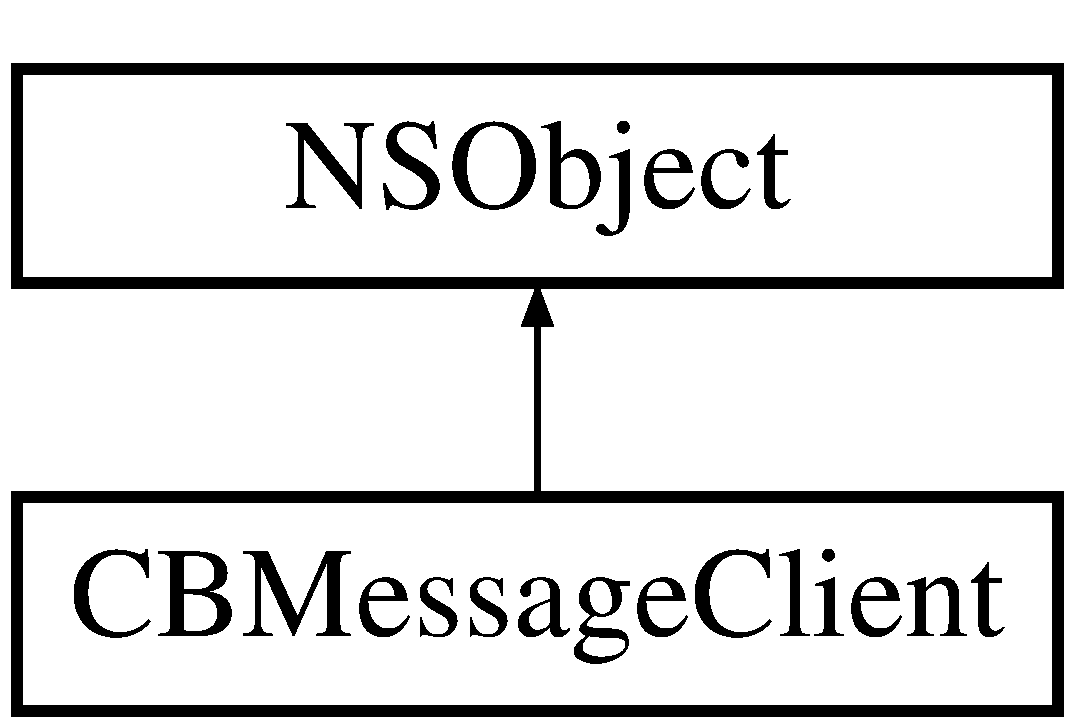
\includegraphics[height=2.000000cm]{interface_c_b_message_client}
\end{center}
\end{figure}
\subsection*{Instance Methods}
\begin{DoxyCompactItemize}
\item 
(void) -\/ \hyperlink{interface_c_b_message_client_a98951fb3c734b7f2dfc4ef3607f54b8d}{connect}
\item 
(void) -\/ \hyperlink{interface_c_b_message_client_ad3fc84eac6cbdef60ee25f5e5a76195f}{connect\+With\+Qo\+S\+:}
\item 
(void) -\/ \hyperlink{interface_c_b_message_client_aacd81270fa332e1a1f534f5ccd51eac8}{disconnect}
\item 
(void) -\/ \hyperlink{interface_c_b_message_client_aa4f3f4ff5be3929038bf6045846738cf}{connect\+To\+Host\+:}
\item 
\hypertarget{interface_c_b_message_client_a783328bc604af291da0d49a8cca8cc26}{(void) -\/ {\bfseries connect\+To\+Host\+:with\+Qo\+S\+:}}\label{interface_c_b_message_client_a783328bc604af291da0d49a8cca8cc26}

\item 
(void) -\/ \hyperlink{interface_c_b_message_client_abcbd056a8bdffbb5c00299343c1b0aeb}{publish\+Message\+:to\+Topic\+:}
\item 
(void) -\/ \hyperlink{interface_c_b_message_client_a5a2d3e7f602801310df4c29fef97c85e}{subscribe\+To\+Topic\+:}
\item 
(void) -\/ \hyperlink{interface_c_b_message_client_a2d09ed72620aad690bbc38a7042106b5}{unsubscribe\+From\+Topic\+:}
\end{DoxyCompactItemize}
\subsection*{Class Methods}
\begin{DoxyCompactItemize}
\item 
(instancetype) + \hyperlink{interface_c_b_message_client_acef3f93cc08d62c70a978d81b04d8f6f}{client}
\end{DoxyCompactItemize}
\subsection*{Properties}
\begin{DoxyCompactItemize}
\item 
id$<$ \hyperlink{protocol_c_b_message_client_delegate-p}{C\+B\+Message\+Client\+Delegate} $>$ \hyperlink{interface_c_b_message_client_a6a94ee89f64cbc4bef855ecdda6fbf85}{delegate}
\item 
bool \hyperlink{interface_c_b_message_client_a6a385330b831471122ffb52b101422fb}{is\+Connected}
\item 
N\+S\+U\+R\+L $\ast$ \hyperlink{interface_c_b_message_client_a770ff8d5b798d220ecc7bc00804112d4}{host}
\item 
N\+S\+Array $\ast$ \hyperlink{interface_c_b_message_client_a41081dc92c32ef8aa7ab364463825398}{topics}
\item 
\hypertarget{interface_c_b_message_client_a735d7e8e3ed831a23e3890cecd45e9e8}{C\+B\+Message\+Client\+Quality {\bfseries qos}}\label{interface_c_b_message_client_a735d7e8e3ed831a23e3890cecd45e9e8}

\end{DoxyCompactItemize}


\subsection{Method Documentation}
\hypertarget{interface_c_b_message_client_acef3f93cc08d62c70a978d81b04d8f6f}{\index{C\+B\+Message\+Client@{C\+B\+Message\+Client}!client@{client}}
\index{client@{client}!CBMessageClient@{C\+B\+Message\+Client}}
\subsubsection[{client}]{\setlength{\rightskip}{0pt plus 5cm}+ (struct mosquitto $\ast$) client 
\begin{DoxyParamCaption}
{}
\end{DoxyParamCaption}
}}\label{interface_c_b_message_client_acef3f93cc08d62c70a978d81b04d8f6f}
Creates a new \hyperlink{interface_c_b_message_client}{C\+B\+Message\+Client} instance. \hypertarget{interface_c_b_message_client_a98951fb3c734b7f2dfc4ef3607f54b8d}{\index{C\+B\+Message\+Client@{C\+B\+Message\+Client}!connect@{connect}}
\index{connect@{connect}!CBMessageClient@{C\+B\+Message\+Client}}
\subsubsection[{connect}]{\setlength{\rightskip}{0pt plus 5cm}-\/ (void) connect 
\begin{DoxyParamCaption}
{}
\end{DoxyParamCaption}
}}\label{interface_c_b_message_client_a98951fb3c734b7f2dfc4ef3607f54b8d}
Connects the client to the default host, specified in \mbox{[}\hyperlink{interface_clear_blade}{Clear\+Blade} settings\mbox{]} \hypertarget{interface_c_b_message_client_aa4f3f4ff5be3929038bf6045846738cf}{\index{C\+B\+Message\+Client@{C\+B\+Message\+Client}!connect\+To\+Host\+:@{connect\+To\+Host\+:}}
\index{connect\+To\+Host\+:@{connect\+To\+Host\+:}!CBMessageClient@{C\+B\+Message\+Client}}
\subsubsection[{connect\+To\+Host\+:}]{\setlength{\rightskip}{0pt plus 5cm}-\/ (void) connect\+To\+Host\+: 
\begin{DoxyParamCaption}
\item[{(N\+S\+U\+R\+L $\ast$)}]{host\+Name}
\end{DoxyParamCaption}
}}\label{interface_c_b_message_client_aa4f3f4ff5be3929038bf6045846738cf}
Connects the client to the host at the specified url. 
\begin{DoxyParams}{Parameters}
{\em host\+Name} & The U\+R\+L to connect to. The U\+R\+L should be of the format tcp\+://address. \\
\hline
\end{DoxyParams}
\hypertarget{interface_c_b_message_client_ad3fc84eac6cbdef60ee25f5e5a76195f}{\index{C\+B\+Message\+Client@{C\+B\+Message\+Client}!connect\+With\+Qo\+S\+:@{connect\+With\+Qo\+S\+:}}
\index{connect\+With\+Qo\+S\+:@{connect\+With\+Qo\+S\+:}!CBMessageClient@{C\+B\+Message\+Client}}
\subsubsection[{connect\+With\+Qo\+S\+:}]{\setlength{\rightskip}{0pt plus 5cm}-\/ (void) connect\+With\+Qo\+S\+: 
\begin{DoxyParamCaption}
\item[{(C\+B\+Message\+Client\+Quality)}]{qos}
\end{DoxyParamCaption}
}}\label{interface_c_b_message_client_ad3fc84eac6cbdef60ee25f5e5a76195f}
Connects the client to the default host, specified in \mbox{[}\hyperlink{interface_clear_blade}{Clear\+Blade} settings\mbox{]}. However, uses the given Quality of Service 
\begin{DoxyParams}{Parameters}
{\em qos} & The Quality of Service of the connection \\
\hline
\end{DoxyParams}
\hypertarget{interface_c_b_message_client_aacd81270fa332e1a1f534f5ccd51eac8}{\index{C\+B\+Message\+Client@{C\+B\+Message\+Client}!disconnect@{disconnect}}
\index{disconnect@{disconnect}!CBMessageClient@{C\+B\+Message\+Client}}
\subsubsection[{disconnect}]{\setlength{\rightskip}{0pt plus 5cm}-\/ (void) disconnect 
\begin{DoxyParamCaption}
{}
\end{DoxyParamCaption}
}}\label{interface_c_b_message_client_aacd81270fa332e1a1f534f5ccd51eac8}
Disconnects the client from it's current server \hypertarget{interface_c_b_message_client_abcbd056a8bdffbb5c00299343c1b0aeb}{\index{C\+B\+Message\+Client@{C\+B\+Message\+Client}!publish\+Message\+:to\+Topic\+:@{publish\+Message\+:to\+Topic\+:}}
\index{publish\+Message\+:to\+Topic\+:@{publish\+Message\+:to\+Topic\+:}!CBMessageClient@{C\+B\+Message\+Client}}
\subsubsection[{publish\+Message\+:to\+Topic\+:}]{\setlength{\rightskip}{0pt plus 5cm}-\/ (void) publish\+Message\+: 
\begin{DoxyParamCaption}
\item[{(N\+S\+String $\ast$)}]{message}
\item[{toTopic:(N\+S\+String $\ast$)}]{topic}
\end{DoxyParamCaption}
}}\label{interface_c_b_message_client_abcbd056a8bdffbb5c00299343c1b0aeb}
Publishs the message client a message to the specified topic. 
\begin{DoxyParams}{Parameters}
{\em message} & The message to send \\
\hline
{\em topic} & The topic to send the message to \\
\hline
\end{DoxyParams}
\hypertarget{interface_c_b_message_client_a5a2d3e7f602801310df4c29fef97c85e}{\index{C\+B\+Message\+Client@{C\+B\+Message\+Client}!subscribe\+To\+Topic\+:@{subscribe\+To\+Topic\+:}}
\index{subscribe\+To\+Topic\+:@{subscribe\+To\+Topic\+:}!CBMessageClient@{C\+B\+Message\+Client}}
\subsubsection[{subscribe\+To\+Topic\+:}]{\setlength{\rightskip}{0pt plus 5cm}-\/ (void) subscribe\+To\+Topic\+: 
\begin{DoxyParamCaption}
\item[{(N\+S\+String $\ast$)}]{topic}
\end{DoxyParamCaption}
}}\label{interface_c_b_message_client_a5a2d3e7f602801310df4c29fef97c85e}
Subscribes the message client to a topic 
\begin{DoxyParams}{Parameters}
{\em topic} & The topic the message client connected to \\
\hline
\end{DoxyParams}
\hypertarget{interface_c_b_message_client_a2d09ed72620aad690bbc38a7042106b5}{\index{C\+B\+Message\+Client@{C\+B\+Message\+Client}!unsubscribe\+From\+Topic\+:@{unsubscribe\+From\+Topic\+:}}
\index{unsubscribe\+From\+Topic\+:@{unsubscribe\+From\+Topic\+:}!CBMessageClient@{C\+B\+Message\+Client}}
\subsubsection[{unsubscribe\+From\+Topic\+:}]{\setlength{\rightskip}{0pt plus 5cm}-\/ (void) unsubscribe\+From\+Topic\+: 
\begin{DoxyParamCaption}
\item[{(N\+S\+String $\ast$)}]{topic}
\end{DoxyParamCaption}
}}\label{interface_c_b_message_client_a2d09ed72620aad690bbc38a7042106b5}
Unsubscribes the message client to a topic 
\begin{DoxyParams}{Parameters}
{\em topic} & The topic to unsubscribe from \\
\hline
\end{DoxyParams}


\subsection{Property Documentation}
\hypertarget{interface_c_b_message_client_a6a94ee89f64cbc4bef855ecdda6fbf85}{\index{C\+B\+Message\+Client@{C\+B\+Message\+Client}!delegate@{delegate}}
\index{delegate@{delegate}!CBMessageClient@{C\+B\+Message\+Client}}
\subsubsection[{delegate}]{\setlength{\rightskip}{0pt plus 5cm}-\/ (id$<${\bf C\+B\+Message\+Client\+Delegate}$>$) delegate\hspace{0.3cm}{\ttfamily [read]}, {\ttfamily [write]}, {\ttfamily [atomic]}, {\ttfamily [weak]}}}\label{interface_c_b_message_client_a6a94ee89f64cbc4bef855ecdda6fbf85}
The delegate that will handle all events from message client \hypertarget{interface_c_b_message_client_a770ff8d5b798d220ecc7bc00804112d4}{\index{C\+B\+Message\+Client@{C\+B\+Message\+Client}!host@{host}}
\index{host@{host}!CBMessageClient@{C\+B\+Message\+Client}}
\subsubsection[{host}]{\setlength{\rightskip}{0pt plus 5cm}-\/ (N\+S\+U\+R\+L $\ast$) host\hspace{0.3cm}{\ttfamily [read]}, {\ttfamily [atomic]}, {\ttfamily [assign]}}}\label{interface_c_b_message_client_a770ff8d5b798d220ecc7bc00804112d4}
The host that this client is connected to. \hypertarget{interface_c_b_message_client_a6a385330b831471122ffb52b101422fb}{\index{C\+B\+Message\+Client@{C\+B\+Message\+Client}!is\+Connected@{is\+Connected}}
\index{is\+Connected@{is\+Connected}!CBMessageClient@{C\+B\+Message\+Client}}
\subsubsection[{is\+Connected}]{\setlength{\rightskip}{0pt plus 5cm}-\/ (bool) is\+Connected\hspace{0.3cm}{\ttfamily [read]}, {\ttfamily [atomic]}, {\ttfamily [assign]}}}\label{interface_c_b_message_client_a6a385330b831471122ffb52b101422fb}
Whether or not this message client is connected to a host \hypertarget{interface_c_b_message_client_a41081dc92c32ef8aa7ab364463825398}{\index{C\+B\+Message\+Client@{C\+B\+Message\+Client}!topics@{topics}}
\index{topics@{topics}!CBMessageClient@{C\+B\+Message\+Client}}
\subsubsection[{topics}]{\setlength{\rightskip}{0pt plus 5cm}-\/ (N\+S\+Array $\ast$) topics\hspace{0.3cm}{\ttfamily [read]}, {\ttfamily [atomic]}, {\ttfamily [assign]}}}\label{interface_c_b_message_client_a41081dc92c32ef8aa7ab364463825398}
The list of topics this client is currently subscribed to 

The documentation for this class was generated from the following files\+:\begin{DoxyCompactItemize}
\item 
C\+B\+Message\+Client.\+h\item 
C\+B\+Message\+Client.\+m\end{DoxyCompactItemize}

\hypertarget{category_c_b_message_client_07_08}{\section{C\+B\+Message\+Client() Category Reference}
\label{category_c_b_message_client_07_08}\index{C\+B\+Message\+Client()@{C\+B\+Message\+Client()}}
}
\subsection*{Instance Methods}
\begin{DoxyCompactItemize}
\item 
\hypertarget{category_c_b_message_client_07_08_a8796e44a34e000a06b70041e686bc3bf}{(void) -\/ {\bfseries handle\+Connect\+:}}\label{category_c_b_message_client_07_08_a8796e44a34e000a06b70041e686bc3bf}

\item 
\hypertarget{category_c_b_message_client_07_08_addb1b9213a29dd815c97f705c0865517}{(void) -\/ {\bfseries handle\+Disconnect}}\label{category_c_b_message_client_07_08_addb1b9213a29dd815c97f705c0865517}

\item 
\hypertarget{category_c_b_message_client_07_08_a03b88809c4e42eca1fc342322d44ea3a}{(void) -\/ {\bfseries handle\+Message\+:}}\label{category_c_b_message_client_07_08_a03b88809c4e42eca1fc342322d44ea3a}

\item 
\hypertarget{category_c_b_message_client_07_08_a7c1d0cd4811c5f45aa53bcf18d0faca6}{(void) -\/ {\bfseries handle\+Publish\+:}}\label{category_c_b_message_client_07_08_a7c1d0cd4811c5f45aa53bcf18d0faca6}

\item 
\hypertarget{category_c_b_message_client_07_08_acf8440144373221fb951c279aa3e6038}{(void) -\/ {\bfseries handle\+Subscribe\+:}}\label{category_c_b_message_client_07_08_acf8440144373221fb951c279aa3e6038}

\item 
\hypertarget{category_c_b_message_client_07_08_a6adf38012722dcfb31bf46dd272e6c1c}{(void) -\/ {\bfseries handle\+Unsubscribe\+:}}\label{category_c_b_message_client_07_08_a6adf38012722dcfb31bf46dd272e6c1c}

\item 
\hypertarget{category_c_b_message_client_07_08_a1254860feec88da1f96fdcebc1f5464d}{(int) -\/ {\bfseries add\+Item\+To\+Message\+Queue\+:}}\label{category_c_b_message_client_07_08_a1254860feec88da1f96fdcebc1f5464d}

\item 
\hypertarget{category_c_b_message_client_07_08_a34249db2f5f6b23c0f6d241fe455317d}{(id) -\/ {\bfseries remove\+Item\+From\+Message\+Queue\+:}}\label{category_c_b_message_client_07_08_a34249db2f5f6b23c0f6d241fe455317d}

\item 
\hypertarget{category_c_b_message_client_07_08_ab3c1c9ba04e5ca719766d9d8745900b8}{(void) -\/ {\bfseries add\+Topic\+To\+Subscribe\+List\+:}}\label{category_c_b_message_client_07_08_ab3c1c9ba04e5ca719766d9d8745900b8}

\item 
\hypertarget{category_c_b_message_client_07_08_a358c4b546f0f1fc96b053957907546dd}{(void) -\/ {\bfseries remove\+Topic\+From\+Subscribe\+List\+:}}\label{category_c_b_message_client_07_08_a358c4b546f0f1fc96b053957907546dd}

\end{DoxyCompactItemize}
\subsection*{Properties}
\begin{DoxyCompactItemize}
\item 
\hypertarget{category_c_b_message_client_07_08_a6dd8044dd2d87c74a8274dd2d772d18c}{struct mosquitto $\ast$ {\bfseries client}}\label{category_c_b_message_client_07_08_a6dd8044dd2d87c74a8274dd2d772d18c}

\item 
\hypertarget{category_c_b_message_client_07_08_a8ea5e9fc7bd6109f0e0bf0a5149ce281}{N\+S\+Object $\ast$ {\bfseries client\+Lock}}\label{category_c_b_message_client_07_08_a8ea5e9fc7bd6109f0e0bf0a5149ce281}

\item 
\hypertarget{category_c_b_message_client_07_08_a352f0fd7c3c5b009801f1d5164fe684f}{N\+S\+Mutable\+Set $\ast$ {\bfseries topic\+List}}\label{category_c_b_message_client_07_08_a352f0fd7c3c5b009801f1d5164fe684f}

\item 
\hypertarget{category_c_b_message_client_07_08_a084c1c0326a36184f673f698eb82cd34}{N\+S\+Mutable\+Dictionary $\ast$ {\bfseries message\+Queue}}\label{category_c_b_message_client_07_08_a084c1c0326a36184f673f698eb82cd34}

\item 
\hypertarget{category_c_b_message_client_07_08_ab510d95792c9d50028d6fa2d34a1a995}{N\+S\+Thread $\ast$ {\bfseries client\+Thread}}\label{category_c_b_message_client_07_08_ab510d95792c9d50028d6fa2d34a1a995}

\item 
\hypertarget{category_c_b_message_client_07_08_a481825e10342415caf9e0f592b606bc5}{N\+S\+Number $\ast$ {\bfseries is\+Connected\+Container}}\label{category_c_b_message_client_07_08_a481825e10342415caf9e0f592b606bc5}

\item 
\hypertarget{category_c_b_message_client_07_08_a7f10d284507cb889192b0a8ea8de88cc}{C\+B\+Message\+Client\+Quality {\bfseries qos}}\label{category_c_b_message_client_07_08_a7f10d284507cb889192b0a8ea8de88cc}

\end{DoxyCompactItemize}


The documentation for this category was generated from the following file\+:\begin{DoxyCompactItemize}
\item 
C\+B\+Message\+Client.\+m\end{DoxyCompactItemize}

\hypertarget{protocol_c_b_message_client_delegate-p}{\section{$<$C\-B\-Message\-Client\-Delegate$>$ Protocol Reference}
\label{protocol_c_b_message_client_delegate-p}\index{$<$\-C\-B\-Message\-Client\-Delegate$>$@{$<$\-C\-B\-Message\-Client\-Delegate$>$}}
}
Inheritance diagram for $<$C\-B\-Message\-Client\-Delegate$>$\-:\begin{figure}[H]
\begin{center}
\leavevmode
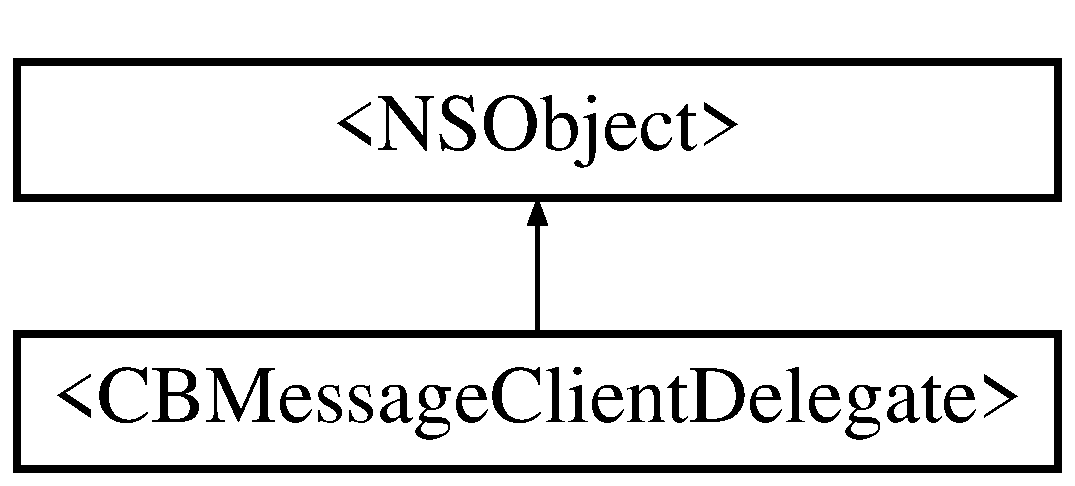
\includegraphics[height=2.000000cm]{protocol_c_b_message_client_delegate-p}
\end{center}
\end{figure}
\subsection*{Instance Methods}
\begin{DoxyCompactItemize}
\item 
\hypertarget{protocol_c_b_message_client_delegate-p_a867359ed1027be7ddfd607a548e3ba96}{(void) -\/ {\bfseries message\-Client\-:did\-Connect\-:}}\label{protocol_c_b_message_client_delegate-p_a867359ed1027be7ddfd607a548e3ba96}

\item 
\hypertarget{protocol_c_b_message_client_delegate-p_a561503ecf3dfabb58045d5ce2a872866}{(void) -\/ {\bfseries message\-Client\-Did\-Disconnect\-:}}\label{protocol_c_b_message_client_delegate-p_a561503ecf3dfabb58045d5ce2a872866}

\item 
\hypertarget{protocol_c_b_message_client_delegate-p_a176ec5e85afee0e0277b70ffb4b4979e}{(void) -\/ {\bfseries message\-Client\-:did\-Publish\-:}}\label{protocol_c_b_message_client_delegate-p_a176ec5e85afee0e0277b70ffb4b4979e}

\item 
\hypertarget{protocol_c_b_message_client_delegate-p_a7b462fdbc23f08496107696bbe84f580}{(void) -\/ {\bfseries message\-Client\-:did\-Receive\-Message\-:}}\label{protocol_c_b_message_client_delegate-p_a7b462fdbc23f08496107696bbe84f580}

\item 
\hypertarget{protocol_c_b_message_client_delegate-p_acdd39cc46ad4e0fcf0b9d5369d358b87}{(void) -\/ {\bfseries message\-Client\-:did\-Subscribe\-:}}\label{protocol_c_b_message_client_delegate-p_acdd39cc46ad4e0fcf0b9d5369d358b87}

\item 
\hypertarget{protocol_c_b_message_client_delegate-p_abf3a4f817617e81ecc7e4c8ae714bc46}{(void) -\/ {\bfseries message\-Client\-:did\-Unsubscribe\-:}}\label{protocol_c_b_message_client_delegate-p_abf3a4f817617e81ecc7e4c8ae714bc46}

\item 
\hypertarget{protocol_c_b_message_client_delegate-p_ae655148c101c94f59c118b765efa9513}{(void) -\/ {\bfseries message\-Client\-:did\-Fail\-To\-Connect\-:}}\label{protocol_c_b_message_client_delegate-p_ae655148c101c94f59c118b765efa9513}

\end{DoxyCompactItemize}


The documentation for this protocol was generated from the following file\-:\begin{DoxyCompactItemize}
\item 
C\-B\-Message\-Client.\-h\end{DoxyCompactItemize}

\hypertarget{interface_c_b_query}{\section{C\+B\+Query Class Reference}
\label{interface_c_b_query}\index{C\+B\+Query@{C\+B\+Query}}
}


{\ttfamily \#import $<$C\+B\+Query.\+h$>$}

Inheritance diagram for C\+B\+Query\+:\begin{figure}[H]
\begin{center}
\leavevmode
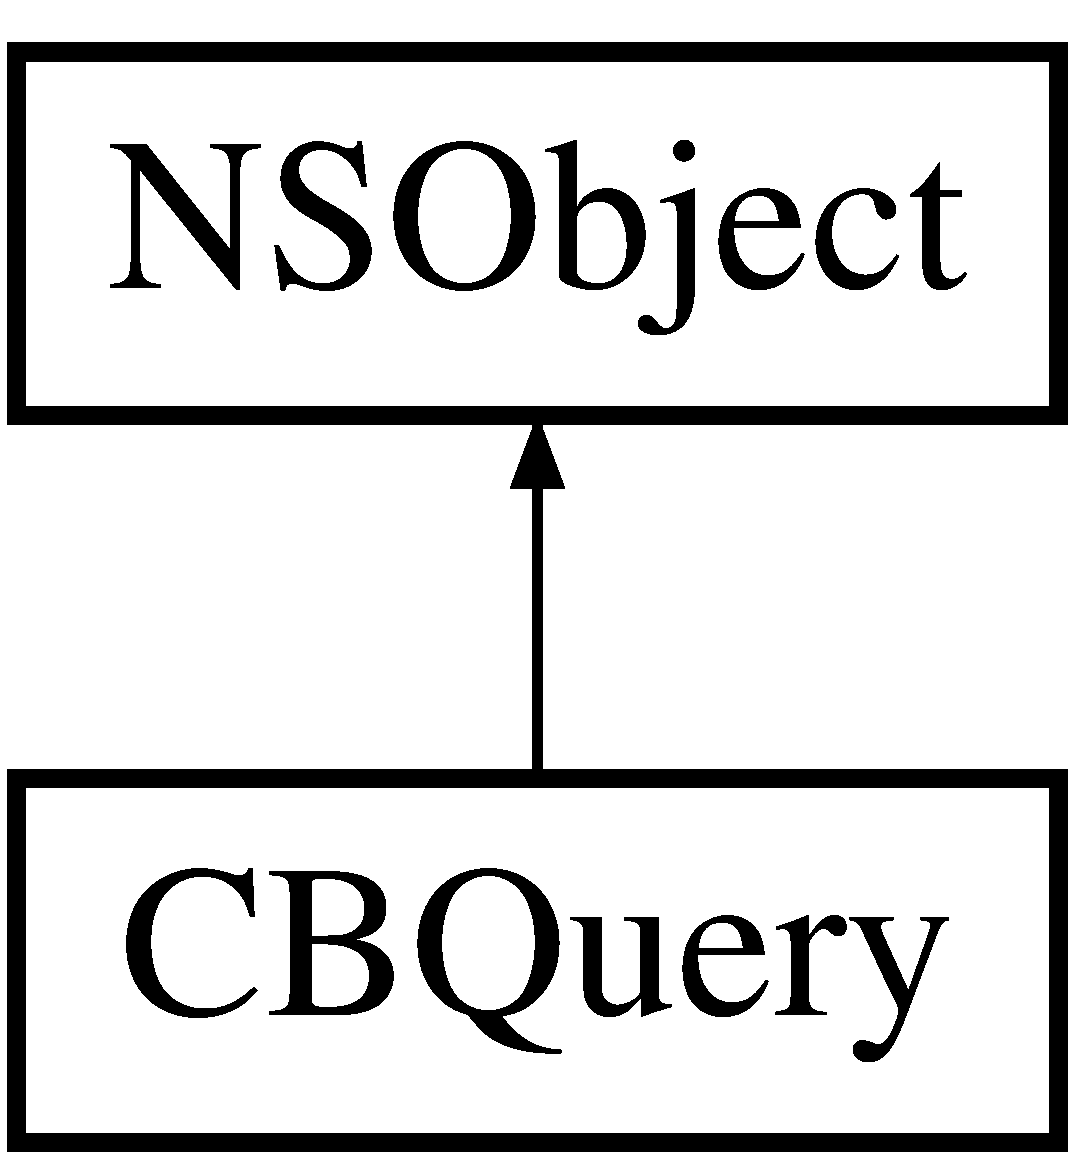
\includegraphics[height=2.000000cm]{interface_c_b_query}
\end{center}
\end{figure}
\subsection*{Instance Methods}
\begin{DoxyCompactItemize}
\item 
(\hyperlink{interface_c_b_query}{C\+B\+Query} $\ast$) -\/ \hyperlink{interface_c_b_query_a945b8a169282151a97e6a0fd694cbb33}{init\+With\+Collection\+I\+D\+:}
\item 
(void) -\/ \hyperlink{interface_c_b_query_aa6df57d4b22629273cb22d39157ab234}{set\+Collection\+I\+D\+:}
\item 
(void) -\/ \hyperlink{interface_c_b_query_a2ff55cfdc8420ce06c3bfe334691a7cd}{fetch\+With\+Success\+Callback\+:with\+Error\+Callback\+:}
\item 
(void) -\/ \hyperlink{interface_c_b_query_aca3f69cedd6770da3fac14535b050d6c}{update\+With\+Changes\+:with\+Success\+Callback\+:with\+Error\+Callback\+:}
\item 
(void) -\/ \hyperlink{interface_c_b_query_a7c2529e9ef2e4c3630b01d8bff1ea25b}{insert\+Item\+:into\+Collection\+With\+I\+D\+:with\+Success\+Callback\+:with\+Error\+Callback\+:}
\item 
(void) -\/ \hyperlink{interface_c_b_query_acecf2b37deaf04803066830664b81ad1}{remove\+With\+Success\+Callback\+:with\+Error\+Callback\+:}
\item 
(\hyperlink{interface_c_b_query}{C\+B\+Query} $\ast$) -\/ \hyperlink{interface_c_b_query_a3ff649bb71392f2f21e210f07f0ef761}{equal\+To\+:for\+:}
\item 
(\hyperlink{interface_c_b_query}{C\+B\+Query} $\ast$) -\/ \hyperlink{interface_c_b_query_af7920062116379d99531b3443a8c3aa3}{not\+Equal\+To\+:for\+:}
\item 
(\hyperlink{interface_c_b_query}{C\+B\+Query} $\ast$) -\/ \hyperlink{interface_c_b_query_a26d58f8c51997aea862c26cc291d743e}{greater\+Than\+:for\+:}
\item 
(\hyperlink{interface_c_b_query}{C\+B\+Query} $\ast$) -\/ \hyperlink{interface_c_b_query_a29af545dcdf721cae1534c219a991021}{less\+Than\+:for\+:}
\item 
(\hyperlink{interface_c_b_query}{C\+B\+Query} $\ast$) -\/ \hyperlink{interface_c_b_query_a52b23279069fa19429ed6473ecf0eb73}{greater\+Than\+Equal\+To\+:for\+:}
\item 
(\hyperlink{interface_c_b_query}{C\+B\+Query} $\ast$) -\/ \hyperlink{interface_c_b_query_ac8007f263dbc069970ee76c90666b043}{less\+Than\+Equal\+To\+:for\+:}
\item 
(\hyperlink{interface_c_b_query}{C\+B\+Query} $\ast$) -\/ \hyperlink{interface_c_b_query_a5d7977f390caeb0eccb620ddf6e24c2f}{set\+Page\+Size\+:}
\item 
(\hyperlink{interface_c_b_query}{C\+B\+Query} $\ast$) -\/ \hyperlink{interface_c_b_query_a04a966e136634595b92597e8437ff176}{set\+Page\+Num\+:}
\item 
(\hyperlink{interface_c_b_query}{C\+B\+Query} $\ast$) -\/ \hyperlink{interface_c_b_query_abcb133d3ea6c27ccd85fc9d1278f7f41}{add\+Query\+As\+Or\+Clause\+Using\+Query\+:}
\end{DoxyCompactItemize}
\subsection*{Class Methods}
\begin{DoxyCompactItemize}
\item 
(\hyperlink{interface_c_b_query}{C\+B\+Query} $\ast$) + \hyperlink{interface_c_b_query_a616541706465f78433a3b2488760df4f}{query\+With\+Collection\+I\+D\+:}
\end{DoxyCompactItemize}
\subsection*{Properties}
\begin{DoxyCompactItemize}
\item 
N\+S\+String $\ast$ \hyperlink{interface_c_b_query_ad7e594dc30699c9dbae407e55b588b00}{collection\+I\+D}
\item 
\hyperlink{interface_c_b_user}{C\+B\+User} $\ast$ \hyperlink{interface_c_b_query_af5679b48acc1313cab6dd83e2777b440}{user}
\end{DoxyCompactItemize}


\subsection{Detailed Description}
Class representing a query that can be used in operations on Platform 

\subsection{Method Documentation}
\hypertarget{interface_c_b_query_abcb133d3ea6c27ccd85fc9d1278f7f41}{\index{C\+B\+Query@{C\+B\+Query}!add\+Query\+As\+Or\+Clause\+Using\+Query\+:@{add\+Query\+As\+Or\+Clause\+Using\+Query\+:}}
\index{add\+Query\+As\+Or\+Clause\+Using\+Query\+:@{add\+Query\+As\+Or\+Clause\+Using\+Query\+:}!CBQuery@{C\+B\+Query}}
\subsubsection[{add\+Query\+As\+Or\+Clause\+Using\+Query\+:}]{\setlength{\rightskip}{0pt plus 5cm}-\/ ({\bf C\+B\+Query} $\ast$) add\+Query\+As\+Or\+Clause\+Using\+Query\+: 
\begin{DoxyParamCaption}
\item[{({\bf C\+B\+Query} $\ast$)}]{or\+Query}
\end{DoxyParamCaption}
}}\label{interface_c_b_query_abcb133d3ea6c27ccd85fc9d1278f7f41}
Adds another \hyperlink{interface_c_b_query}{C\+B\+Query} as an O\+R clause. This allows you to create two separate \hyperlink{interface_c_b_query}{C\+B\+Query} objects to then O\+R together. This operation happens in place so the caller's underlying query is changed but the Query used as the argument is not. 
\begin{DoxyParams}{Parameters}
{\em or\+Query} & A \hyperlink{interface_c_b_query}{C\+B\+Query} to be O\+R'd to the calling \hyperlink{interface_c_b_query}{C\+B\+Query}.\\
\hline
\end{DoxyParams}
Example\+: \hyperlink{interface_c_b_query}{C\+B\+Query} $\ast$first\+Query = \mbox{[}\hyperlink{interface_c_b_query}{C\+B\+Query} query\+With\+Collection\+I\+D\+:"f28faaa10a8ca5a5f2f5acd297cc01\char`\"{}\mbox{]}
\mbox{[}first\+Query equal\+To\+:@\char`\"{}value1\char`\"{} for\+:@\char`\"{}key1\char`\"{}\mbox{]}
\mbox{[}first\+Query equal\+To\+:@\char`\"{}value2\char`\"{} for\+:@\char`\"{}key2\char`\"{}\mbox{]}
\+C\+B\+Query $\ast$second\+Query = \mbox{[}\+C\+B\+Query query\+With\+Collection\+I\+D\+:@\char`\"{}f28faaa10a8ca5a5f2f5acd297cc01\char`\"{}\mbox{]}
\mbox{[}second\+Query equal\+To@\char`\"{}value3\char`\"{} for\+:@\char`\"{}key3"\mbox{]} \hyperlink{interface_c_b_query}{C\+B\+Query} $\ast$third\+Query = \mbox{[}first\+Query add\+Query\+As\+Or\+Clause\+Using\+Query\+:second\+Query\mbox{]}

In the example, third\+Query would be equivalent to this S\+Q\+L\+: W\+H\+E\+R\+E \char`\"{}key1\char`\"{} = \char`\"{}value1\char`\"{} A\+N\+D \char`\"{}key2\char`\"{} = \char`\"{}value2\char`\"{} O\+R \char`\"{}key3\char`\"{} = \char`\"{}value3\char`\"{} \hypertarget{interface_c_b_query_a3ff649bb71392f2f21e210f07f0ef761}{\index{C\+B\+Query@{C\+B\+Query}!equal\+To\+:for\+:@{equal\+To\+:for\+:}}
\index{equal\+To\+:for\+:@{equal\+To\+:for\+:}!CBQuery@{C\+B\+Query}}
\subsubsection[{equal\+To\+:for\+:}]{\setlength{\rightskip}{0pt plus 5cm}-\/ ({\bf C\+B\+Query} $\ast$) equal\+To\+: 
\begin{DoxyParamCaption}
\item[{(id)}]{value}
\item[{for:(N\+S\+String $\ast$)}]{key}
\end{DoxyParamCaption}
}}\label{interface_c_b_query_a3ff649bb71392f2f21e210f07f0ef761}
Creates an equality clause and adds it to the query 
\begin{DoxyParams}{Parameters}
{\em value} & A string that gets set as the value for the given key \\
\hline
{\em key} & A string that is used as the key for the given value \\
\hline
\end{DoxyParams}
\begin{DoxyReturn}{Returns}
The query with the new clause added 
\end{DoxyReturn}
\hypertarget{interface_c_b_query_a2ff55cfdc8420ce06c3bfe334691a7cd}{\index{C\+B\+Query@{C\+B\+Query}!fetch\+With\+Success\+Callback\+:with\+Error\+Callback\+:@{fetch\+With\+Success\+Callback\+:with\+Error\+Callback\+:}}
\index{fetch\+With\+Success\+Callback\+:with\+Error\+Callback\+:@{fetch\+With\+Success\+Callback\+:with\+Error\+Callback\+:}!CBQuery@{C\+B\+Query}}
\subsubsection[{fetch\+With\+Success\+Callback\+:with\+Error\+Callback\+:}]{\setlength{\rightskip}{0pt plus 5cm}-\/ (void) fetch\+With\+Success\+Callback\+: 
\begin{DoxyParamCaption}
\item[{(C\+B\+Query\+Success\+Callback)}]{success\+Callback}
\item[{withErrorCallback:(C\+B\+Query\+Error\+Callback)}]{failure\+Callback}
\end{DoxyParamCaption}
}}\label{interface_c_b_query_a2ff55cfdc8420ce06c3bfe334691a7cd}
Fetches from a collection all of the items that match the query that is sent. 
\begin{DoxyParams}{Parameters}
{\em success\+Callback} & A callback block that handles the returned data \\
\hline
{\em failure\+Callback} & A callback block that handles errors returned \\
\hline
\end{DoxyParams}
\hypertarget{interface_c_b_query_a26d58f8c51997aea862c26cc291d743e}{\index{C\+B\+Query@{C\+B\+Query}!greater\+Than\+:for\+:@{greater\+Than\+:for\+:}}
\index{greater\+Than\+:for\+:@{greater\+Than\+:for\+:}!CBQuery@{C\+B\+Query}}
\subsubsection[{greater\+Than\+:for\+:}]{\setlength{\rightskip}{0pt plus 5cm}-\/ ({\bf C\+B\+Query} $\ast$) greater\+Than\+: 
\begin{DoxyParamCaption}
\item[{(N\+S\+Number $\ast$)}]{value}
\item[{for:(N\+S\+String $\ast$)}]{key}
\end{DoxyParamCaption}
}}\label{interface_c_b_query_a26d58f8c51997aea862c26cc291d743e}
Creates a greater than clause and adds it to the query 
\begin{DoxyParams}{Parameters}
{\em value} & A string that gets set as the value for the given key \\
\hline
{\em key} & A string that is used as the key for the given value \\
\hline
\end{DoxyParams}
\begin{DoxyReturn}{Returns}
The query with the new clause added 
\end{DoxyReturn}
\hypertarget{interface_c_b_query_a52b23279069fa19429ed6473ecf0eb73}{\index{C\+B\+Query@{C\+B\+Query}!greater\+Than\+Equal\+To\+:for\+:@{greater\+Than\+Equal\+To\+:for\+:}}
\index{greater\+Than\+Equal\+To\+:for\+:@{greater\+Than\+Equal\+To\+:for\+:}!CBQuery@{C\+B\+Query}}
\subsubsection[{greater\+Than\+Equal\+To\+:for\+:}]{\setlength{\rightskip}{0pt plus 5cm}-\/ ({\bf C\+B\+Query} $\ast$) greater\+Than\+Equal\+To\+: 
\begin{DoxyParamCaption}
\item[{(N\+S\+Number $\ast$)}]{value}
\item[{for:(N\+S\+String $\ast$)}]{key}
\end{DoxyParamCaption}
}}\label{interface_c_b_query_a52b23279069fa19429ed6473ecf0eb73}
Creates a greater than or equal to clause and adds it to the query 
\begin{DoxyParams}{Parameters}
{\em value} & A string that gets set as the value for the given key \\
\hline
{\em key} & A string that is used as the key for the given value \\
\hline
\end{DoxyParams}
\begin{DoxyReturn}{Returns}
The query with the new clause added 
\end{DoxyReturn}
\hypertarget{interface_c_b_query_a945b8a169282151a97e6a0fd694cbb33}{\index{C\+B\+Query@{C\+B\+Query}!init\+With\+Collection\+I\+D\+:@{init\+With\+Collection\+I\+D\+:}}
\index{init\+With\+Collection\+I\+D\+:@{init\+With\+Collection\+I\+D\+:}!CBQuery@{C\+B\+Query}}
\subsubsection[{init\+With\+Collection\+I\+D\+:}]{\setlength{\rightskip}{0pt plus 5cm}-\/ ({\bf C\+B\+Query} $\ast$) init\+With\+Collection\+I\+D\+: 
\begin{DoxyParamCaption}
\item[{(N\+S\+String $\ast$)}]{col\+I\+D}
\end{DoxyParamCaption}
}}\label{interface_c_b_query_a945b8a169282151a97e6a0fd694cbb33}
Initializes the query object and sets the collection\+I\+D 
\begin{DoxyParams}{Parameters}
{\em col\+I\+D} & A string that is set as collection\+I\+D \\
\hline
\end{DoxyParams}
\begin{DoxyReturn}{Returns}
the newly instantiated \hyperlink{interface_c_b_query}{C\+B\+Query} Object 
\end{DoxyReturn}
\hypertarget{interface_c_b_query_a7c2529e9ef2e4c3630b01d8bff1ea25b}{\index{C\+B\+Query@{C\+B\+Query}!insert\+Item\+:into\+Collection\+With\+I\+D\+:with\+Success\+Callback\+:with\+Error\+Callback\+:@{insert\+Item\+:into\+Collection\+With\+I\+D\+:with\+Success\+Callback\+:with\+Error\+Callback\+:}}
\index{insert\+Item\+:into\+Collection\+With\+I\+D\+:with\+Success\+Callback\+:with\+Error\+Callback\+:@{insert\+Item\+:into\+Collection\+With\+I\+D\+:with\+Success\+Callback\+:with\+Error\+Callback\+:}!CBQuery@{C\+B\+Query}}
\subsubsection[{insert\+Item\+:into\+Collection\+With\+I\+D\+:with\+Success\+Callback\+:with\+Error\+Callback\+:}]{\setlength{\rightskip}{0pt plus 5cm}-\/ (void) insert\+Item\+: 
\begin{DoxyParamCaption}
\item[{({\bf C\+B\+Item} $\ast$)}]{item}
\item[{intoCollectionWithID:(N\+S\+String $\ast$)}]{collection\+I\+D}
\item[{withSuccessCallback:(C\+B\+Operation\+Success\+Callback)}]{success\+Callback}
\item[{withErrorCallback:(C\+B\+Query\+Error\+Callback)}]{error\+Callback}
\end{DoxyParamCaption}
}}\label{interface_c_b_query_a7c2529e9ef2e4c3630b01d8bff1ea25b}
Inserts the object into the collection. Ignores any query parameters 
\begin{DoxyParams}{Parameters}
{\em item} & The item to be inserted into the collection \\
\hline
{\em collection\+I\+D} & The I\+D of the collection to insert the item into \\
\hline
{\em success\+Callback} & A callback block that handles the return data \\
\hline
{\em error\+Callback} & A callback block that handles the errors returned \\
\hline
\end{DoxyParams}
\hypertarget{interface_c_b_query_a29af545dcdf721cae1534c219a991021}{\index{C\+B\+Query@{C\+B\+Query}!less\+Than\+:for\+:@{less\+Than\+:for\+:}}
\index{less\+Than\+:for\+:@{less\+Than\+:for\+:}!CBQuery@{C\+B\+Query}}
\subsubsection[{less\+Than\+:for\+:}]{\setlength{\rightskip}{0pt plus 5cm}-\/ ({\bf C\+B\+Query} $\ast$) less\+Than\+: 
\begin{DoxyParamCaption}
\item[{(N\+S\+Number $\ast$)}]{value}
\item[{for:(N\+S\+String $\ast$)}]{key}
\end{DoxyParamCaption}
}}\label{interface_c_b_query_a29af545dcdf721cae1534c219a991021}
Creates a less than clause and adds it to the query 
\begin{DoxyParams}{Parameters}
{\em value} & A string that gets set as the value for the given key \\
\hline
{\em key} & A string that is used as the key for the given value \\
\hline
\end{DoxyParams}
\begin{DoxyReturn}{Returns}
The query with the new clause added 
\end{DoxyReturn}
\hypertarget{interface_c_b_query_ac8007f263dbc069970ee76c90666b043}{\index{C\+B\+Query@{C\+B\+Query}!less\+Than\+Equal\+To\+:for\+:@{less\+Than\+Equal\+To\+:for\+:}}
\index{less\+Than\+Equal\+To\+:for\+:@{less\+Than\+Equal\+To\+:for\+:}!CBQuery@{C\+B\+Query}}
\subsubsection[{less\+Than\+Equal\+To\+:for\+:}]{\setlength{\rightskip}{0pt plus 5cm}-\/ ({\bf C\+B\+Query} $\ast$) less\+Than\+Equal\+To\+: 
\begin{DoxyParamCaption}
\item[{(N\+S\+Number $\ast$)}]{value}
\item[{for:(N\+S\+String $\ast$)}]{key}
\end{DoxyParamCaption}
}}\label{interface_c_b_query_ac8007f263dbc069970ee76c90666b043}
Creates a less than or equal to clause and adds it to the query 
\begin{DoxyParams}{Parameters}
{\em value} & A string that gets set as the value for the given key \\
\hline
{\em key} & A string that is used as the key for the given value \\
\hline
\end{DoxyParams}
\begin{DoxyReturn}{Returns}
The query with the new clause added 
\end{DoxyReturn}
\hypertarget{interface_c_b_query_af7920062116379d99531b3443a8c3aa3}{\index{C\+B\+Query@{C\+B\+Query}!not\+Equal\+To\+:for\+:@{not\+Equal\+To\+:for\+:}}
\index{not\+Equal\+To\+:for\+:@{not\+Equal\+To\+:for\+:}!CBQuery@{C\+B\+Query}}
\subsubsection[{not\+Equal\+To\+:for\+:}]{\setlength{\rightskip}{0pt plus 5cm}-\/ ({\bf C\+B\+Query} $\ast$) not\+Equal\+To\+: 
\begin{DoxyParamCaption}
\item[{(id)}]{value}
\item[{for:(N\+S\+String $\ast$)}]{key}
\end{DoxyParamCaption}
}}\label{interface_c_b_query_af7920062116379d99531b3443a8c3aa3}
Creates an inequality clause and adds it to the query 
\begin{DoxyParams}{Parameters}
{\em value} & A string that gets set as the value for the given key \\
\hline
{\em key} & A string that is used as the key for the given value \\
\hline
\end{DoxyParams}
\begin{DoxyReturn}{Returns}
The query with the new clause added 
\end{DoxyReturn}
\hypertarget{interface_c_b_query_a616541706465f78433a3b2488760df4f}{\index{C\+B\+Query@{C\+B\+Query}!query\+With\+Collection\+I\+D\+:@{query\+With\+Collection\+I\+D\+:}}
\index{query\+With\+Collection\+I\+D\+:@{query\+With\+Collection\+I\+D\+:}!CBQuery@{C\+B\+Query}}
\subsubsection[{query\+With\+Collection\+I\+D\+:}]{\setlength{\rightskip}{0pt plus 5cm}+ ({\bf C\+B\+Query} $\ast$) query\+With\+Collection\+I\+D\+: 
\begin{DoxyParamCaption}
\item[{(N\+S\+String $\ast$)}]{collection\+I\+D}
\end{DoxyParamCaption}
}}\label{interface_c_b_query_a616541706465f78433a3b2488760df4f}
Creates a query object that will operate on the collection with the collection\+I\+D \hypertarget{interface_c_b_query_acecf2b37deaf04803066830664b81ad1}{\index{C\+B\+Query@{C\+B\+Query}!remove\+With\+Success\+Callback\+:with\+Error\+Callback\+:@{remove\+With\+Success\+Callback\+:with\+Error\+Callback\+:}}
\index{remove\+With\+Success\+Callback\+:with\+Error\+Callback\+:@{remove\+With\+Success\+Callback\+:with\+Error\+Callback\+:}!CBQuery@{C\+B\+Query}}
\subsubsection[{remove\+With\+Success\+Callback\+:with\+Error\+Callback\+:}]{\setlength{\rightskip}{0pt plus 5cm}-\/ (void) remove\+With\+Success\+Callback\+: 
\begin{DoxyParamCaption}
\item[{(C\+B\+Operation\+Success\+Callback)}]{success\+Callback}
\item[{withErrorCallback:(C\+B\+Query\+Error\+Callback)}]{failure\+Callback}
\end{DoxyParamCaption}
}}\label{interface_c_b_query_acecf2b37deaf04803066830664b81ad1}
Remove from the platform all of the items that match the query sent 
\begin{DoxyParams}{Parameters}
{\em success\+Callback} & A callback block that handles the returned data \\
\hline
{\em failure\+Callback} & A callback block that handles the errors returned \\
\hline
\end{DoxyParams}
\hypertarget{interface_c_b_query_aa6df57d4b22629273cb22d39157ab234}{\index{C\+B\+Query@{C\+B\+Query}!set\+Collection\+I\+D\+:@{set\+Collection\+I\+D\+:}}
\index{set\+Collection\+I\+D\+:@{set\+Collection\+I\+D\+:}!CBQuery@{C\+B\+Query}}
\subsubsection[{set\+Collection\+I\+D\+:}]{\setlength{\rightskip}{0pt plus 5cm}-\/ (void) set\+Collection\+I\+D\+: 
\begin{DoxyParamCaption}
\item[{(N\+S\+String $\ast$)}]{col\+I\+D}
\end{DoxyParamCaption}
}}\label{interface_c_b_query_aa6df57d4b22629273cb22d39157ab234}
Sets the collection I\+D attribute 
\begin{DoxyParams}{Parameters}
{\em col\+I\+D} & A string that will be set as the Collection I\+D \\
\hline
\end{DoxyParams}
\hypertarget{interface_c_b_query_a04a966e136634595b92597e8437ff176}{\index{C\+B\+Query@{C\+B\+Query}!set\+Page\+Num\+:@{set\+Page\+Num\+:}}
\index{set\+Page\+Num\+:@{set\+Page\+Num\+:}!CBQuery@{C\+B\+Query}}
\subsubsection[{set\+Page\+Num\+:}]{\setlength{\rightskip}{0pt plus 5cm}-\/ ({\bf C\+B\+Query} $\ast$) set\+Page\+Num\+: 
\begin{DoxyParamCaption}
\item[{(N\+S\+Number $\ast$)}]{num}
\end{DoxyParamCaption}
}}\label{interface_c_b_query_a04a966e136634595b92597e8437ff176}
Sets the page num for the query that is called 
\begin{DoxyParams}{Parameters}
{\em num} & The page number \\
\hline
\end{DoxyParams}
\begin{DoxyReturn}{Returns}
the query with the page number added 
\end{DoxyReturn}
\hypertarget{interface_c_b_query_a5d7977f390caeb0eccb620ddf6e24c2f}{\index{C\+B\+Query@{C\+B\+Query}!set\+Page\+Size\+:@{set\+Page\+Size\+:}}
\index{set\+Page\+Size\+:@{set\+Page\+Size\+:}!CBQuery@{C\+B\+Query}}
\subsubsection[{set\+Page\+Size\+:}]{\setlength{\rightskip}{0pt plus 5cm}-\/ ({\bf C\+B\+Query} $\ast$) set\+Page\+Size\+: 
\begin{DoxyParamCaption}
\item[{(N\+S\+Number $\ast$)}]{size}
\end{DoxyParamCaption}
}}\label{interface_c_b_query_a5d7977f390caeb0eccb620ddf6e24c2f}
Sets the page size for the query that is called 
\begin{DoxyParams}{Parameters}
{\em size} & The page size \\
\hline
\end{DoxyParams}
\begin{DoxyReturn}{Returns}
The query with the page size added 
\end{DoxyReturn}
\hypertarget{interface_c_b_query_aca3f69cedd6770da3fac14535b050d6c}{\index{C\+B\+Query@{C\+B\+Query}!update\+With\+Changes\+:with\+Success\+Callback\+:with\+Error\+Callback\+:@{update\+With\+Changes\+:with\+Success\+Callback\+:with\+Error\+Callback\+:}}
\index{update\+With\+Changes\+:with\+Success\+Callback\+:with\+Error\+Callback\+:@{update\+With\+Changes\+:with\+Success\+Callback\+:with\+Error\+Callback\+:}!CBQuery@{C\+B\+Query}}
\subsubsection[{update\+With\+Changes\+:with\+Success\+Callback\+:with\+Error\+Callback\+:}]{\setlength{\rightskip}{0pt plus 5cm}-\/ (void) update\+With\+Changes\+: 
\begin{DoxyParamCaption}
\item[{(N\+S\+Dictionary $\ast$)}]{changes}
\item[{withSuccessCallback:(C\+B\+Operation\+Success\+Callback)}]{success\+Callback}
\item[{withErrorCallback:(C\+B\+Query\+Error\+Callback)}]{failure\+Callback}
\end{DoxyParamCaption}
}}\label{interface_c_b_query_aca3f69cedd6770da3fac14535b050d6c}
Updates on the platform all the items that match the query sent 
\begin{DoxyParams}{Parameters}
{\em changes} & A dictoinary of all the changes that will be applied to the items that match the query \\
\hline
{\em success\+Callback} & A callback block that handles the returned data \\
\hline
{\em failure\+Callback} & A callback block that handles the errors returned \\
\hline
\end{DoxyParams}


\subsection{Property Documentation}
\hypertarget{interface_c_b_query_ad7e594dc30699c9dbae407e55b588b00}{\index{C\+B\+Query@{C\+B\+Query}!collection\+I\+D@{collection\+I\+D}}
\index{collection\+I\+D@{collection\+I\+D}!CBQuery@{C\+B\+Query}}
\subsubsection[{collection\+I\+D}]{\setlength{\rightskip}{0pt plus 5cm}-\/ (N\+S\+String$\ast$) collection\+I\+D\hspace{0.3cm}{\ttfamily [read]}, {\ttfamily [write]}, {\ttfamily [nonatomic]}, {\ttfamily [strong]}}}\label{interface_c_b_query_ad7e594dc30699c9dbae407e55b588b00}
The string that represent the I\+D of the collection that will be queried \hypertarget{interface_c_b_query_af5679b48acc1313cab6dd83e2777b440}{\index{C\+B\+Query@{C\+B\+Query}!user@{user}}
\index{user@{user}!CBQuery@{C\+B\+Query}}
\subsubsection[{user}]{\setlength{\rightskip}{0pt plus 5cm}-\/ ({\bf C\+B\+User} $\ast$) user\hspace{0.3cm}{\ttfamily [read]}, {\ttfamily [write]}, {\ttfamily [nonatomic]}, {\ttfamily [strong]}}}\label{interface_c_b_query_af5679b48acc1313cab6dd83e2777b440}
The user that is making the query. It defaults to \mbox{[}Clearblade settings\mbox{]}.main\+User. 

The documentation for this class was generated from the following files\+:\begin{DoxyCompactItemize}
\item 
C\+B\+Query.\+h\item 
C\+B\+Query.\+m\end{DoxyCompactItemize}

\hypertarget{category_c_b_query_07_08}{\section{C\+B\+Query() Category Reference}
\label{category_c_b_query_07_08}\index{C\+B\+Query()@{C\+B\+Query()}}
}
\subsection*{Instance Methods}
\begin{DoxyCompactItemize}
\item 
\hypertarget{category_c_b_query_07_08_abec846bf09cf27bb81de57485416d516}{(N\+S\+Dictionary $\ast$) -\/ {\bfseries dictionary\+Values\+To\+Strings\+:}}\label{category_c_b_query_07_08_abec846bf09cf27bb81de57485416d516}

\end{DoxyCompactItemize}
\subsection*{Properties}
\begin{DoxyCompactItemize}
\item 
\hypertarget{category_c_b_query_07_08_a44c199651c37b422ba5d9b2ee0f70150}{N\+S\+Mutable\+Dictionary $\ast$ {\bfseries query}}\label{category_c_b_query_07_08_a44c199651c37b422ba5d9b2ee0f70150}

\item 
\hypertarget{category_c_b_query_07_08_add581855d14363fa3de237576f8fbb57}{N\+S\+Mutable\+Array $\ast$ {\bfseries O\+R}}\label{category_c_b_query_07_08_add581855d14363fa3de237576f8fbb57}

\end{DoxyCompactItemize}


The documentation for this category was generated from the following file\+:\begin{DoxyCompactItemize}
\item 
Clear\+Blade\+A\+P\+I/C\+B\+Query.\+m\end{DoxyCompactItemize}

\hypertarget{interface_c_b_user}{\section{C\+B\+User Class Reference}
\label{interface_c_b_user}\index{C\+B\+User@{C\+B\+User}}
}


{\ttfamily \#import $<$C\+B\+User.\+h$>$}

Inheritance diagram for C\+B\+User\+:\begin{figure}[H]
\begin{center}
\leavevmode
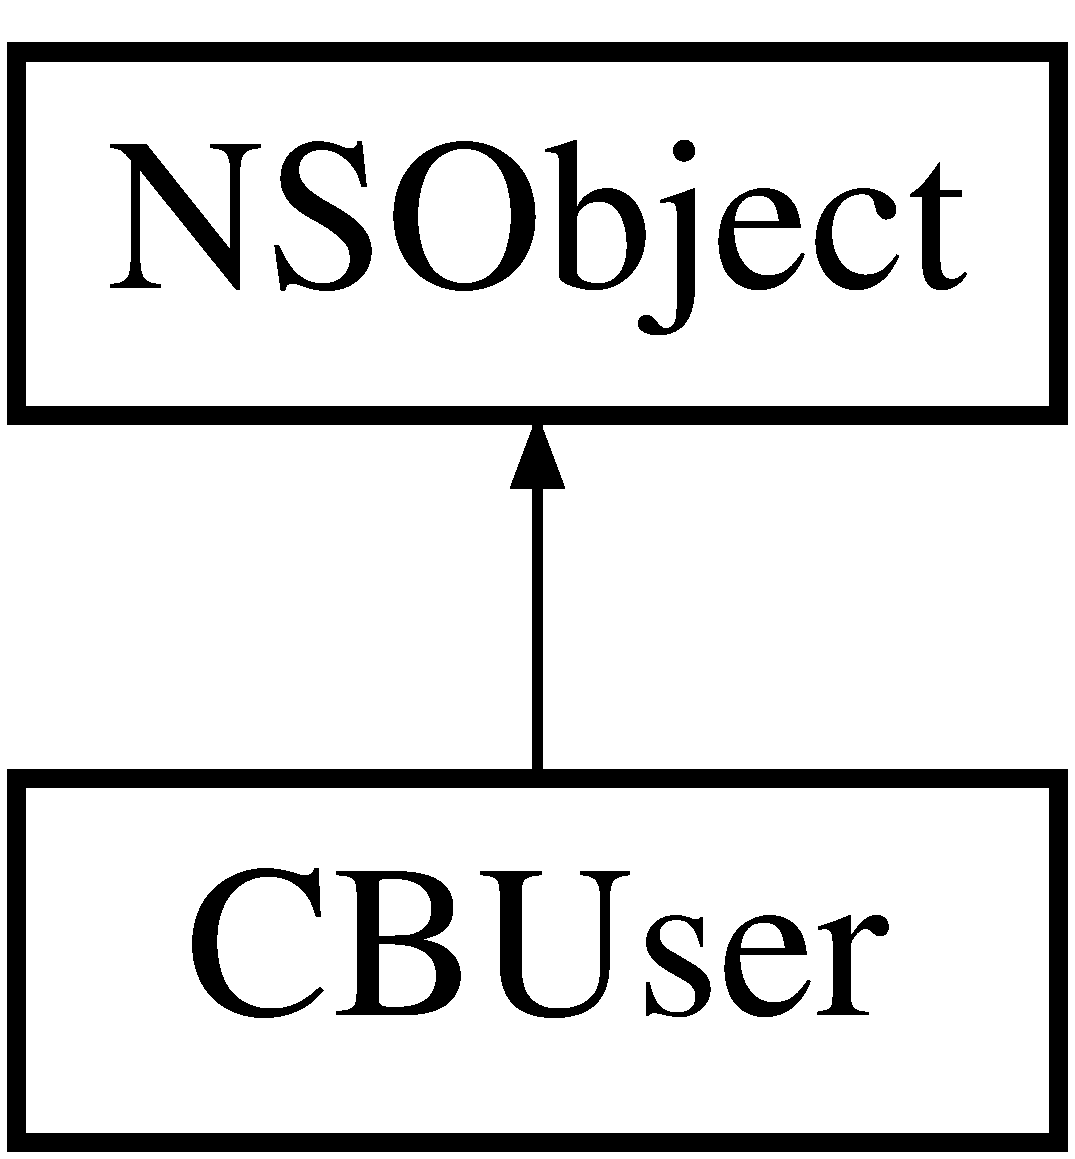
\includegraphics[height=2.000000cm]{interface_c_b_user}
\end{center}
\end{figure}
\subsection*{Instance Methods}
\begin{DoxyCompactItemize}
\item 
(bool) -\/ \hyperlink{interface_c_b_user_a28b25fbf031ecb81c531e6a003ccf766}{check\+Is\+Valid\+With\+Server\+With\+Error\+:}
\item 
(void) -\/ \hyperlink{interface_c_b_user_ab423b6cd05f2db5f6835e886088c83d6}{check\+Is\+Valid\+With\+Server\+With\+Callback\+:with\+Error\+Callback\+:}
\item 
(bool) -\/ \hyperlink{interface_c_b_user_a06f36a7260297c2b191ed2f6e98e43fa}{log\+Out\+With\+Error\+:}
\item 
(void) -\/ \hyperlink{interface_c_b_user_a8deee144e1e7fbc6e1b4c8522a59921e}{log\+Out\+With\+Success\+Callback\+:with\+Error\+Callback\+:}
\end{DoxyCompactItemize}
\subsection*{Class Methods}
\begin{DoxyCompactItemize}
\item 
(instancetype) + \hyperlink{interface_c_b_user_af932ff5e8e7cf2614e223b8bb1040e5d}{anonymous\+User\+With\+Auth\+Token\+:}
\item 
(instancetype) + \hyperlink{interface_c_b_user_ac45cec16ef019ff7d160864c0b73b3a3}{authenticated\+User\+With\+Email\+:with\+Auth\+Token\+:}
\item 
(instancetype) + \hyperlink{interface_c_b_user_a3196760e01e3215f93cd2fab8e515bc9}{authenticate\+User\+With\+Email\+:with\+Password\+:with\+Error\+:}
\item 
(instancetype) + \hyperlink{interface_c_b_user_adab8bc298bccc0892dbb431b3bd6b72e}{authenticate\+User\+With\+Settings\+:with\+Email\+:with\+Password\+:with\+Error\+:}
\item 
(instancetype) + \hyperlink{interface_c_b_user_a87de9d5282ea3a1b1f400cc5e31a8100}{register\+User\+With\+Email\+:with\+Password\+:with\+Error\+:}
\item 
(instancetype) + \hyperlink{interface_c_b_user_a8ee4f3073a9360c5829abb300234477c}{register\+User\+With\+Settings\+:with\+Email\+:with\+Password\+:with\+Error\+:}
\item 
(void) + \hyperlink{interface_c_b_user_a00b1b4b1ba436b1081b92d9c50d42da0}{authenticate\+User\+With\+Email\+:with\+Password\+:with\+Success\+Callback\+:with\+Error\+Callback\+:}
\item 
(void) + \hyperlink{interface_c_b_user_ad4295bcc046be1b9b988f52757e6253b}{authenticate\+User\+With\+Settings\+:with\+Email\+:with\+Password\+:with\+Success\+Callback\+:with\+Error\+Callback\+:}
\item 
(void) + \hyperlink{interface_c_b_user_a3b2eced573b27bdc4bbf6d1401cc74d9}{register\+User\+With\+Email\+:with\+Password\+:with\+Success\+Callback\+:with\+Error\+Callback\+:}
\item 
(void) + \hyperlink{interface_c_b_user_a5cd8d3c8cabe7988dc70237903bafae9}{register\+User\+With\+Settings\+:with\+Email\+:with\+Password\+:with\+Success\+Callback\+:with\+Error\+Callback\+:}
\item 
(\hyperlink{interface_c_b_user}{C\+B\+User} $\ast$) + \hyperlink{interface_c_b_user_aaa5d3708c50ffc320fb80c92faeba4ef}{anonymous\+User\+With\+Settings\+:\+With\+Error\+:}
\item 
(void) + \hyperlink{interface_c_b_user_a177e50a6f6fd1bae2e9bae9a6ad073e6}{anonymous\+User\+With\+Settings\+:with\+Success\+Callback\+:with\+Error\+Callback\+:}
\end{DoxyCompactItemize}
\subsection*{Properties}
\begin{DoxyCompactItemize}
\item 
B\+O\+O\+L \hyperlink{interface_c_b_user_a50094838fe6cca3581124412ed588b51}{is\+Anonymous}
\item 
N\+S\+String $\ast$ \hyperlink{interface_c_b_user_a7907af25f66ea43d5b53ca0e70df34a2}{email}
\item 
N\+S\+String $\ast$ \hyperlink{interface_c_b_user_a942ca51689b5cfc7f8dc740f7543f54a}{auth\+Token}
\end{DoxyCompactItemize}


\subsection{Detailed Description}
Represents a user authenticated into the platform. Can be used directly on requests, or can be applied globally to requests using \mbox{[}\mbox{[}\hyperlink{interface_clear_blade}{Clear\+Blade} settings\mbox{]} set\+Main\+User\+:\mbox{]} 

\subsection{Method Documentation}
\hypertarget{interface_c_b_user_af932ff5e8e7cf2614e223b8bb1040e5d}{\index{C\+B\+User@{C\+B\+User}!anonymous\+User\+With\+Auth\+Token\+:@{anonymous\+User\+With\+Auth\+Token\+:}}
\index{anonymous\+User\+With\+Auth\+Token\+:@{anonymous\+User\+With\+Auth\+Token\+:}!CBUser@{C\+B\+User}}
\subsubsection[{anonymous\+User\+With\+Auth\+Token\+:}]{\setlength{\rightskip}{0pt plus 5cm}+ (instancetype) anonymous\+User\+With\+Auth\+Token\+: 
\begin{DoxyParamCaption}
\item[{(N\+S\+String $\ast$)}]{auth\+Token}
\end{DoxyParamCaption}
}}\label{interface_c_b_user_af932ff5e8e7cf2614e223b8bb1040e5d}
Creates an anonymous user with the specified auth token. This does not communicate with the server in any way to validate the token. 
\begin{DoxyParams}{Parameters}
{\em auth\+Token} & The authorization token to use \\
\hline
\end{DoxyParams}
\begin{DoxyReturn}{Returns}
A User object with an anonymous user using the specified auth\+Token 
\end{DoxyReturn}
\hypertarget{interface_c_b_user_aaa5d3708c50ffc320fb80c92faeba4ef}{\index{C\+B\+User@{C\+B\+User}!anonymous\+User\+With\+Settings\+:\+With\+Error\+:@{anonymous\+User\+With\+Settings\+:\+With\+Error\+:}}
\index{anonymous\+User\+With\+Settings\+:\+With\+Error\+:@{anonymous\+User\+With\+Settings\+:\+With\+Error\+:}!CBUser@{C\+B\+User}}
\subsubsection[{anonymous\+User\+With\+Settings\+:\+With\+Error\+:}]{\setlength{\rightskip}{0pt plus 5cm}+ ({\bf C\+B\+User} $\ast$) anonymous\+User\+With\+Settings\+: 
\begin{DoxyParamCaption}
\item[{({\bf Clear\+Blade} $\ast$)}]{settings}
\item[{WithError:(N\+S\+Error $\ast$$\ast$)}]{error}
\end{DoxyParamCaption}
}}\label{interface_c_b_user_aaa5d3708c50ffc320fb80c92faeba4ef}
Requests an anonynomous user token from the server synchronously. 
\begin{DoxyParams}{Parameters}
{\em settings} & The \hyperlink{interface_clear_blade}{Clear\+Blade} settings object to use. If nil, will just use the default address \\
\hline
{\em error} & Set if there's any issue with requesting the user token. \\
\hline
\end{DoxyParams}
\begin{DoxyReturn}{Returns}
The newly created anonymous user. 
\end{DoxyReturn}
\hypertarget{interface_c_b_user_a177e50a6f6fd1bae2e9bae9a6ad073e6}{\index{C\+B\+User@{C\+B\+User}!anonymous\+User\+With\+Settings\+:with\+Success\+Callback\+:with\+Error\+Callback\+:@{anonymous\+User\+With\+Settings\+:with\+Success\+Callback\+:with\+Error\+Callback\+:}}
\index{anonymous\+User\+With\+Settings\+:with\+Success\+Callback\+:with\+Error\+Callback\+:@{anonymous\+User\+With\+Settings\+:with\+Success\+Callback\+:with\+Error\+Callback\+:}!CBUser@{C\+B\+User}}
\subsubsection[{anonymous\+User\+With\+Settings\+:with\+Success\+Callback\+:with\+Error\+Callback\+:}]{\setlength{\rightskip}{0pt plus 5cm}+ (void) anonymous\+User\+With\+Settings\+: 
\begin{DoxyParamCaption}
\item[{({\bf Clear\+Blade} $\ast$)}]{settings}
\item[{withSuccessCallback:(C\+B\+User\+Success\+Callback)}]{success\+Callback}
\item[{withErrorCallback:(C\+B\+User\+Error\+Callback)}]{error\+Callback}
\end{DoxyParamCaption}
}}\label{interface_c_b_user_a177e50a6f6fd1bae2e9bae9a6ad073e6}
Request an anonymous user token from the server asynchronously. 
\begin{DoxyParams}{Parameters}
{\em settings} & The \hyperlink{interface_clear_blade}{Clear\+Blade} settings object to use. If nil, will just use the default address \\
\hline
{\em Success\+Callback} & Called with the user when the anonymous user is successfully created from the server \\
\hline
{\em Error\+Callback} & Called if any issue while creating the anonymous user arrises. \\
\hline
\end{DoxyParams}
\hypertarget{interface_c_b_user_ac45cec16ef019ff7d160864c0b73b3a3}{\index{C\+B\+User@{C\+B\+User}!authenticated\+User\+With\+Email\+:with\+Auth\+Token\+:@{authenticated\+User\+With\+Email\+:with\+Auth\+Token\+:}}
\index{authenticated\+User\+With\+Email\+:with\+Auth\+Token\+:@{authenticated\+User\+With\+Email\+:with\+Auth\+Token\+:}!CBUser@{C\+B\+User}}
\subsubsection[{authenticated\+User\+With\+Email\+:with\+Auth\+Token\+:}]{\setlength{\rightskip}{0pt plus 5cm}+ (instancetype) authenticated\+User\+With\+Email\+: 
\begin{DoxyParamCaption}
\item[{(N\+S\+String $\ast$)}]{email}
\item[{withAuthToken:(N\+S\+String $\ast$)}]{auth\+Token}
\end{DoxyParamCaption}
}}\label{interface_c_b_user_ac45cec16ef019ff7d160864c0b73b3a3}
Creates a named user with the specified email and auth token. This does not communicate with the server in any way to validate the token, or the email. Currently there is not a way to verify that the email is attached to the auth\+Token, but you can verify that the auth\+Token at least is valid through the selector check\+Is\+Valid\+With\+Server\+Sync\+With\+Error\+: 
\begin{DoxyParams}{Parameters}
{\em Email} & The email the user has \\
\hline
{\em auth\+Token} & The auth token associated with that email \\
\hline
\end{DoxyParams}
\begin{DoxyReturn}{Returns}
A User object with the specified email and auth\+Token. 
\end{DoxyReturn}
\hypertarget{interface_c_b_user_a3196760e01e3215f93cd2fab8e515bc9}{\index{C\+B\+User@{C\+B\+User}!authenticate\+User\+With\+Email\+:with\+Password\+:with\+Error\+:@{authenticate\+User\+With\+Email\+:with\+Password\+:with\+Error\+:}}
\index{authenticate\+User\+With\+Email\+:with\+Password\+:with\+Error\+:@{authenticate\+User\+With\+Email\+:with\+Password\+:with\+Error\+:}!CBUser@{C\+B\+User}}
\subsubsection[{authenticate\+User\+With\+Email\+:with\+Password\+:with\+Error\+:}]{\setlength{\rightskip}{0pt plus 5cm}+ (instancetype) authenticate\+User\+With\+Email\+: 
\begin{DoxyParamCaption}
\item[{(N\+S\+String $\ast$)}]{email}
\item[{withPassword:(N\+S\+String $\ast$)}]{password}
\item[{withError:(N\+S\+Error $\ast$$\ast$)}]{error}
\end{DoxyParamCaption}
}}\label{interface_c_b_user_a3196760e01e3215f93cd2fab8e515bc9}
Authenticates a user with the specified email and password. It retrieves the user's token from the server synchronously, and does not store the password locally. 
\begin{DoxyParams}{Parameters}
{\em email} & The email to create the user with \\
\hline
{\em password} & The password to use \\
\hline
{\em error} & A pointer to the error if there was an issue authenticating the user. \\
\hline
\end{DoxyParams}
\begin{DoxyReturn}{Returns}
The newly created user 
\end{DoxyReturn}
\hypertarget{interface_c_b_user_a00b1b4b1ba436b1081b92d9c50d42da0}{\index{C\+B\+User@{C\+B\+User}!authenticate\+User\+With\+Email\+:with\+Password\+:with\+Success\+Callback\+:with\+Error\+Callback\+:@{authenticate\+User\+With\+Email\+:with\+Password\+:with\+Success\+Callback\+:with\+Error\+Callback\+:}}
\index{authenticate\+User\+With\+Email\+:with\+Password\+:with\+Success\+Callback\+:with\+Error\+Callback\+:@{authenticate\+User\+With\+Email\+:with\+Password\+:with\+Success\+Callback\+:with\+Error\+Callback\+:}!CBUser@{C\+B\+User}}
\subsubsection[{authenticate\+User\+With\+Email\+:with\+Password\+:with\+Success\+Callback\+:with\+Error\+Callback\+:}]{\setlength{\rightskip}{0pt plus 5cm}+ (void) authenticate\+User\+With\+Email\+: 
\begin{DoxyParamCaption}
\item[{(N\+S\+String $\ast$)}]{email}
\item[{withPassword:(N\+S\+String $\ast$)}]{password}
\item[{withSuccessCallback:(C\+B\+User\+Success\+Callback)}]{success\+Callback}
\item[{withErrorCallback:(C\+B\+User\+Error\+Callback)}]{error\+Callback}
\end{DoxyParamCaption}
}}\label{interface_c_b_user_a00b1b4b1ba436b1081b92d9c50d42da0}
Authenticates a user with the specified email and password. It retrieves the user's token from the server asynchronously and calls the callback once the user is authenticated, and does not store the password locally. 
\begin{DoxyParams}{Parameters}
{\em email} & The email to create the user with \\
\hline
{\em password} & The password to use \\
\hline
{\em success\+Callback} & The callback that handles a successful authentication \\
\hline
{\em error\+Callback} & The callback that handles a failed authentication \\
\hline
\end{DoxyParams}
\hypertarget{interface_c_b_user_adab8bc298bccc0892dbb431b3bd6b72e}{\index{C\+B\+User@{C\+B\+User}!authenticate\+User\+With\+Settings\+:with\+Email\+:with\+Password\+:with\+Error\+:@{authenticate\+User\+With\+Settings\+:with\+Email\+:with\+Password\+:with\+Error\+:}}
\index{authenticate\+User\+With\+Settings\+:with\+Email\+:with\+Password\+:with\+Error\+:@{authenticate\+User\+With\+Settings\+:with\+Email\+:with\+Password\+:with\+Error\+:}!CBUser@{C\+B\+User}}
\subsubsection[{authenticate\+User\+With\+Settings\+:with\+Email\+:with\+Password\+:with\+Error\+:}]{\setlength{\rightskip}{0pt plus 5cm}+ (instancetype) authenticate\+User\+With\+Settings\+: 
\begin{DoxyParamCaption}
\item[{({\bf Clear\+Blade} $\ast$)}]{settings}
\item[{withEmail:(N\+S\+String $\ast$)}]{email}
\item[{withPassword:(N\+S\+String $\ast$)}]{password}
\item[{withError:(N\+S\+Error $\ast$$\ast$)}]{error}
\end{DoxyParamCaption}
}}\label{interface_c_b_user_adab8bc298bccc0892dbb431b3bd6b72e}
Authenticates a user with the specified email and password. It retrieves the user's token from the server synchronusly, and does not store the password locally. Uses the specified settings object for the server Address 
\begin{DoxyParams}{Parameters}
{\em settings} & The settings to use to lookup the platform \\
\hline
{\em email} & The email to create the user with \\
\hline
{\em password} & The password to use \\
\hline
{\em error} & A pointer to the error if there was an issue authenticating the user. \\
\hline
\end{DoxyParams}
\begin{DoxyReturn}{Returns}
The newly created user 
\end{DoxyReturn}
\hypertarget{interface_c_b_user_ad4295bcc046be1b9b988f52757e6253b}{\index{C\+B\+User@{C\+B\+User}!authenticate\+User\+With\+Settings\+:with\+Email\+:with\+Password\+:with\+Success\+Callback\+:with\+Error\+Callback\+:@{authenticate\+User\+With\+Settings\+:with\+Email\+:with\+Password\+:with\+Success\+Callback\+:with\+Error\+Callback\+:}}
\index{authenticate\+User\+With\+Settings\+:with\+Email\+:with\+Password\+:with\+Success\+Callback\+:with\+Error\+Callback\+:@{authenticate\+User\+With\+Settings\+:with\+Email\+:with\+Password\+:with\+Success\+Callback\+:with\+Error\+Callback\+:}!CBUser@{C\+B\+User}}
\subsubsection[{authenticate\+User\+With\+Settings\+:with\+Email\+:with\+Password\+:with\+Success\+Callback\+:with\+Error\+Callback\+:}]{\setlength{\rightskip}{0pt plus 5cm}+ (void) authenticate\+User\+With\+Settings\+: 
\begin{DoxyParamCaption}
\item[{({\bf Clear\+Blade} $\ast$)}]{settings}
\item[{withEmail:(N\+S\+String $\ast$)}]{email}
\item[{withPassword:(N\+S\+String $\ast$)}]{password}
\item[{withSuccessCallback:(C\+B\+User\+Success\+Callback)}]{success\+Callback}
\item[{withErrorCallback:(C\+B\+User\+Error\+Callback)}]{error\+Callback}
\end{DoxyParamCaption}
}}\label{interface_c_b_user_ad4295bcc046be1b9b988f52757e6253b}
Authenticates a user with the specified email and password. It retrieves the user's token from the server synchronusly, and does not store the password locally. Uses the specified settings object for the server Address 
\begin{DoxyParams}{Parameters}
{\em settings} & The settings to use to lookup the platform \\
\hline
{\em email} & The email to create the user with \\
\hline
{\em password} & The password to use \\
\hline
{\em success\+Callback} & The callback that handles a successful authentication \\
\hline
{\em error\+Callback} & The callback that handles a failed authentication \\
\hline
\end{DoxyParams}
\hypertarget{interface_c_b_user_ab423b6cd05f2db5f6835e886088c83d6}{\index{C\+B\+User@{C\+B\+User}!check\+Is\+Valid\+With\+Server\+With\+Callback\+:with\+Error\+Callback\+:@{check\+Is\+Valid\+With\+Server\+With\+Callback\+:with\+Error\+Callback\+:}}
\index{check\+Is\+Valid\+With\+Server\+With\+Callback\+:with\+Error\+Callback\+:@{check\+Is\+Valid\+With\+Server\+With\+Callback\+:with\+Error\+Callback\+:}!CBUser@{C\+B\+User}}
\subsubsection[{check\+Is\+Valid\+With\+Server\+With\+Callback\+:with\+Error\+Callback\+:}]{\setlength{\rightskip}{0pt plus 5cm}-\/ (void) check\+Is\+Valid\+With\+Server\+With\+Callback\+: 
\begin{DoxyParamCaption}
\item[{(C\+B\+User\+Is\+Valid\+Callback)}]{is\+Valid\+Callback}
\item[{withErrorCallback:(C\+B\+User\+Error\+Callback)}]{error\+Callback}
\end{DoxyParamCaption}
}}\label{interface_c_b_user_ab423b6cd05f2db5f6835e886088c83d6}
Checks if the user token is still valid with server asynchronously. Error callback is only called if there is an issue communicating with the server 
\begin{DoxyParams}{Parameters}
{\em is\+Valid\+Callback} & Has a true boolean if the server thinks it's a valid token, false if the server thinks it is not \\
\hline
{\em error\+Callback} & Only called if there is an issue communicating with the server \\
\hline
\end{DoxyParams}
\hypertarget{interface_c_b_user_a28b25fbf031ecb81c531e6a003ccf766}{\index{C\+B\+User@{C\+B\+User}!check\+Is\+Valid\+With\+Server\+With\+Error\+:@{check\+Is\+Valid\+With\+Server\+With\+Error\+:}}
\index{check\+Is\+Valid\+With\+Server\+With\+Error\+:@{check\+Is\+Valid\+With\+Server\+With\+Error\+:}!CBUser@{C\+B\+User}}
\subsubsection[{check\+Is\+Valid\+With\+Server\+With\+Error\+:}]{\setlength{\rightskip}{0pt plus 5cm}-\/ (bool) check\+Is\+Valid\+With\+Server\+With\+Error\+: 
\begin{DoxyParamCaption}
\item[{(N\+S\+Error $\ast$$\ast$)}]{error}
\end{DoxyParamCaption}
}}\label{interface_c_b_user_a28b25fbf031ecb81c531e6a003ccf766}
Checks if the user token is still valid with server synchronously. Error is only set if there is an issue communicating with the server 
\begin{DoxyParams}{Parameters}
{\em error} & The error if there's an issue communicating with server \\
\hline
\end{DoxyParams}
\begin{DoxyReturn}{Returns}
True if the server thinks it's a valid token, false if the server thinks it is not. 
\end{DoxyReturn}
\hypertarget{interface_c_b_user_a06f36a7260297c2b191ed2f6e98e43fa}{\index{C\+B\+User@{C\+B\+User}!log\+Out\+With\+Error\+:@{log\+Out\+With\+Error\+:}}
\index{log\+Out\+With\+Error\+:@{log\+Out\+With\+Error\+:}!CBUser@{C\+B\+User}}
\subsubsection[{log\+Out\+With\+Error\+:}]{\setlength{\rightskip}{0pt plus 5cm}-\/ (bool) log\+Out\+With\+Error\+: 
\begin{DoxyParamCaption}
\item[{(N\+S\+Error $\ast$$\ast$)}]{error}
\end{DoxyParamCaption}
}}\label{interface_c_b_user_a06f36a7260297c2b191ed2f6e98e43fa}
Logs the user with the token out of the server synchronously. 
\begin{DoxyParams}{Parameters}
{\em error} & If there's any error logging the user out, including if the user's token is already logged out \\
\hline
\end{DoxyParams}
\begin{DoxyReturn}{Returns}
Returns true if there's no error 
\end{DoxyReturn}
\hypertarget{interface_c_b_user_a8deee144e1e7fbc6e1b4c8522a59921e}{\index{C\+B\+User@{C\+B\+User}!log\+Out\+With\+Success\+Callback\+:with\+Error\+Callback\+:@{log\+Out\+With\+Success\+Callback\+:with\+Error\+Callback\+:}}
\index{log\+Out\+With\+Success\+Callback\+:with\+Error\+Callback\+:@{log\+Out\+With\+Success\+Callback\+:with\+Error\+Callback\+:}!CBUser@{C\+B\+User}}
\subsubsection[{log\+Out\+With\+Success\+Callback\+:with\+Error\+Callback\+:}]{\setlength{\rightskip}{0pt plus 5cm}-\/ (void) log\+Out\+With\+Success\+Callback\+: 
\begin{DoxyParamCaption}
\item[{(void($^\wedge$)())}]{success\+Callback}
\item[{withErrorCallback:(C\+B\+User\+Error\+Callback)}]{error\+Callback}
\end{DoxyParamCaption}
}}\label{interface_c_b_user_a8deee144e1e7fbc6e1b4c8522a59921e}
Logs the user with the token out of the server asynchronously. 
\begin{DoxyParams}{Parameters}
{\em Success\+Callback} & Called if the user is logged out successfully. \\
\hline
{\em Error\+Callback} & Called if there is any error logging the user out, including if the user's token is already logged out \\
\hline
\end{DoxyParams}
\hypertarget{interface_c_b_user_a87de9d5282ea3a1b1f400cc5e31a8100}{\index{C\+B\+User@{C\+B\+User}!register\+User\+With\+Email\+:with\+Password\+:with\+Error\+:@{register\+User\+With\+Email\+:with\+Password\+:with\+Error\+:}}
\index{register\+User\+With\+Email\+:with\+Password\+:with\+Error\+:@{register\+User\+With\+Email\+:with\+Password\+:with\+Error\+:}!CBUser@{C\+B\+User}}
\subsubsection[{register\+User\+With\+Email\+:with\+Password\+:with\+Error\+:}]{\setlength{\rightskip}{0pt plus 5cm}+ (instancetype) register\+User\+With\+Email\+: 
\begin{DoxyParamCaption}
\item[{(N\+S\+String $\ast$)}]{email}
\item[{withPassword:(N\+S\+String $\ast$)}]{password}
\item[{withError:(N\+S\+Error $\ast$$\ast$)}]{error}
\end{DoxyParamCaption}
}}\label{interface_c_b_user_a87de9d5282ea3a1b1f400cc5e31a8100}
Registers a user with the specified email and password. It retrieves the user's token from the server synchronously, and does not store the password locally. 
\begin{DoxyParams}{Parameters}
{\em email} & The email to create the user with \\
\hline
{\em password} & The password to use \\
\hline
{\em error} & A pointer to the error if there was an issue registering the user. \\
\hline
\end{DoxyParams}
\begin{DoxyReturn}{Returns}
The newly created user 
\end{DoxyReturn}
\hypertarget{interface_c_b_user_a3b2eced573b27bdc4bbf6d1401cc74d9}{\index{C\+B\+User@{C\+B\+User}!register\+User\+With\+Email\+:with\+Password\+:with\+Success\+Callback\+:with\+Error\+Callback\+:@{register\+User\+With\+Email\+:with\+Password\+:with\+Success\+Callback\+:with\+Error\+Callback\+:}}
\index{register\+User\+With\+Email\+:with\+Password\+:with\+Success\+Callback\+:with\+Error\+Callback\+:@{register\+User\+With\+Email\+:with\+Password\+:with\+Success\+Callback\+:with\+Error\+Callback\+:}!CBUser@{C\+B\+User}}
\subsubsection[{register\+User\+With\+Email\+:with\+Password\+:with\+Success\+Callback\+:with\+Error\+Callback\+:}]{\setlength{\rightskip}{0pt plus 5cm}+ (void) register\+User\+With\+Email\+: 
\begin{DoxyParamCaption}
\item[{(N\+S\+String $\ast$)}]{email}
\item[{withPassword:(N\+S\+String $\ast$)}]{password}
\item[{withSuccessCallback:(C\+B\+User\+Success\+Callback)}]{success\+Callback}
\item[{withErrorCallback:(C\+B\+User\+Error\+Callback)}]{error\+Callback}
\end{DoxyParamCaption}
}}\label{interface_c_b_user_a3b2eced573b27bdc4bbf6d1401cc74d9}
Registers a user with the specified email and password. It retrieves the user's token from the server asynchronously and calls the callback once the user is authenticated, and does not store the password locally. 
\begin{DoxyParams}{Parameters}
{\em email} & The email to create the user with \\
\hline
{\em password} & The password to use \\
\hline
{\em success\+Callback} & The callback that handles a successful register \\
\hline
{\em error\+Callback} & The callback that handles a failed register \\
\hline
\end{DoxyParams}
\begin{DoxyReturn}{Returns}
The newly created user 
\end{DoxyReturn}
\hypertarget{interface_c_b_user_a8ee4f3073a9360c5829abb300234477c}{\index{C\+B\+User@{C\+B\+User}!register\+User\+With\+Settings\+:with\+Email\+:with\+Password\+:with\+Error\+:@{register\+User\+With\+Settings\+:with\+Email\+:with\+Password\+:with\+Error\+:}}
\index{register\+User\+With\+Settings\+:with\+Email\+:with\+Password\+:with\+Error\+:@{register\+User\+With\+Settings\+:with\+Email\+:with\+Password\+:with\+Error\+:}!CBUser@{C\+B\+User}}
\subsubsection[{register\+User\+With\+Settings\+:with\+Email\+:with\+Password\+:with\+Error\+:}]{\setlength{\rightskip}{0pt plus 5cm}+ (instancetype) register\+User\+With\+Settings\+: 
\begin{DoxyParamCaption}
\item[{({\bf Clear\+Blade} $\ast$)}]{settings}
\item[{withEmail:(N\+S\+String $\ast$)}]{email}
\item[{withPassword:(N\+S\+String $\ast$)}]{password}
\item[{withError:(N\+S\+Error $\ast$$\ast$)}]{error}
\end{DoxyParamCaption}
}}\label{interface_c_b_user_a8ee4f3073a9360c5829abb300234477c}
Registers a user with the specified email and password. It retrieves the user's token from the server synchronously, and does not store the password locally. 
\begin{DoxyParams}{Parameters}
{\em settings} & The settings to use to lookup the platform \\
\hline
{\em email} & The email to create the user with \\
\hline
{\em password} & The password to use \\
\hline
{\em error} & A pointer to the error if there was an issue registering the user. \\
\hline
\end{DoxyParams}
\begin{DoxyReturn}{Returns}
The newly created user 
\end{DoxyReturn}
\hypertarget{interface_c_b_user_a5cd8d3c8cabe7988dc70237903bafae9}{\index{C\+B\+User@{C\+B\+User}!register\+User\+With\+Settings\+:with\+Email\+:with\+Password\+:with\+Success\+Callback\+:with\+Error\+Callback\+:@{register\+User\+With\+Settings\+:with\+Email\+:with\+Password\+:with\+Success\+Callback\+:with\+Error\+Callback\+:}}
\index{register\+User\+With\+Settings\+:with\+Email\+:with\+Password\+:with\+Success\+Callback\+:with\+Error\+Callback\+:@{register\+User\+With\+Settings\+:with\+Email\+:with\+Password\+:with\+Success\+Callback\+:with\+Error\+Callback\+:}!CBUser@{C\+B\+User}}
\subsubsection[{register\+User\+With\+Settings\+:with\+Email\+:with\+Password\+:with\+Success\+Callback\+:with\+Error\+Callback\+:}]{\setlength{\rightskip}{0pt plus 5cm}+ (void) register\+User\+With\+Settings\+: 
\begin{DoxyParamCaption}
\item[{({\bf Clear\+Blade} $\ast$)}]{settings}
\item[{withEmail:(N\+S\+String $\ast$)}]{email}
\item[{withPassword:(N\+S\+String $\ast$)}]{password}
\item[{withSuccessCallback:(C\+B\+User\+Success\+Callback)}]{success\+Callback}
\item[{withErrorCallback:(C\+B\+User\+Error\+Callback)}]{error\+Callback}
\end{DoxyParamCaption}
}}\label{interface_c_b_user_a5cd8d3c8cabe7988dc70237903bafae9}
Registers a user with the specified email and password. It retrieves the user's token from the server asynchronously and calls the callback once the user is authenticated, and does not store the password locally. Uses the specified settings object for the server Address 
\begin{DoxyParams}{Parameters}
{\em settings} & The settings to use to lookup the platform \\
\hline
{\em email} & The email to create the user with \\
\hline
{\em password} & The password to use \\
\hline
{\em success\+Callback} & The callback that handles a successful register \\
\hline
{\em error\+Callback} & The callback that handles a failed register \\
\hline
\end{DoxyParams}
\begin{DoxyReturn}{Returns}
The newly created user 
\end{DoxyReturn}


\subsection{Property Documentation}
\hypertarget{interface_c_b_user_a942ca51689b5cfc7f8dc740f7543f54a}{\index{C\+B\+User@{C\+B\+User}!auth\+Token@{auth\+Token}}
\index{auth\+Token@{auth\+Token}!CBUser@{C\+B\+User}}
\subsubsection[{auth\+Token}]{\setlength{\rightskip}{0pt plus 5cm}-\/ (N\+S\+String$\ast$) auth\+Token\hspace{0.3cm}{\ttfamily [read]}, {\ttfamily [nonatomic]}, {\ttfamily [strong]}}}\label{interface_c_b_user_a942ca51689b5cfc7f8dc740f7543f54a}
The token from the server used to identify the user in requests \hypertarget{interface_c_b_user_a7907af25f66ea43d5b53ca0e70df34a2}{\index{C\+B\+User@{C\+B\+User}!email@{email}}
\index{email@{email}!CBUser@{C\+B\+User}}
\subsubsection[{email}]{\setlength{\rightskip}{0pt plus 5cm}-\/ (N\+S\+String$\ast$) email\hspace{0.3cm}{\ttfamily [read]}, {\ttfamily [nonatomic]}, {\ttfamily [strong]}}}\label{interface_c_b_user_a7907af25f66ea43d5b53ca0e70df34a2}
The email identifying the user \hypertarget{interface_c_b_user_a50094838fe6cca3581124412ed588b51}{\index{C\+B\+User@{C\+B\+User}!is\+Anonymous@{is\+Anonymous}}
\index{is\+Anonymous@{is\+Anonymous}!CBUser@{C\+B\+User}}
\subsubsection[{is\+Anonymous}]{\setlength{\rightskip}{0pt plus 5cm}-\/ (B\+O\+O\+L) is\+Anonymous\hspace{0.3cm}{\ttfamily [read]}, {\ttfamily [write]}, {\ttfamily [atomic]}, {\ttfamily [assign]}}}\label{interface_c_b_user_a50094838fe6cca3581124412ed588b51}
Is true if the user has no email or password, and is just an anonymous token from the server 

The documentation for this class was generated from the following files\+:\begin{DoxyCompactItemize}
\item 
C\+B\+User.\+h\item 
C\+B\+User.\+m\end{DoxyCompactItemize}

\hypertarget{category_c_b_user_07_08}{\section{C\+B\+User() Category Reference}
\label{category_c_b_user_07_08}\index{C\+B\+User()@{C\+B\+User()}}
}
\subsection*{Properties}
\begin{DoxyCompactItemize}
\item 
\hypertarget{category_c_b_user_07_08_a9bdf5fd8da471de347bc15f06e362d2b}{N\+S\+String $\ast$ {\bfseries email}}\label{category_c_b_user_07_08_a9bdf5fd8da471de347bc15f06e362d2b}

\item 
\hypertarget{category_c_b_user_07_08_afb9f1f9c2826ad9a138e63ec3bffe1fc}{N\+S\+String $\ast$ {\bfseries auth\+Token}}\label{category_c_b_user_07_08_afb9f1f9c2826ad9a138e63ec3bffe1fc}

\end{DoxyCompactItemize}


The documentation for this category was generated from the following file\+:\begin{DoxyCompactItemize}
\item 
C\+B\+User.\+m\end{DoxyCompactItemize}

\hypertarget{interface_clear_blade}{\section{Clear\+Blade Class Reference}
\label{interface_clear_blade}\index{Clear\+Blade@{Clear\+Blade}}
}


{\ttfamily \#import $<$Clear\+Blade.\+h$>$}

Inheritance diagram for Clear\+Blade\+:\begin{figure}[H]
\begin{center}
\leavevmode
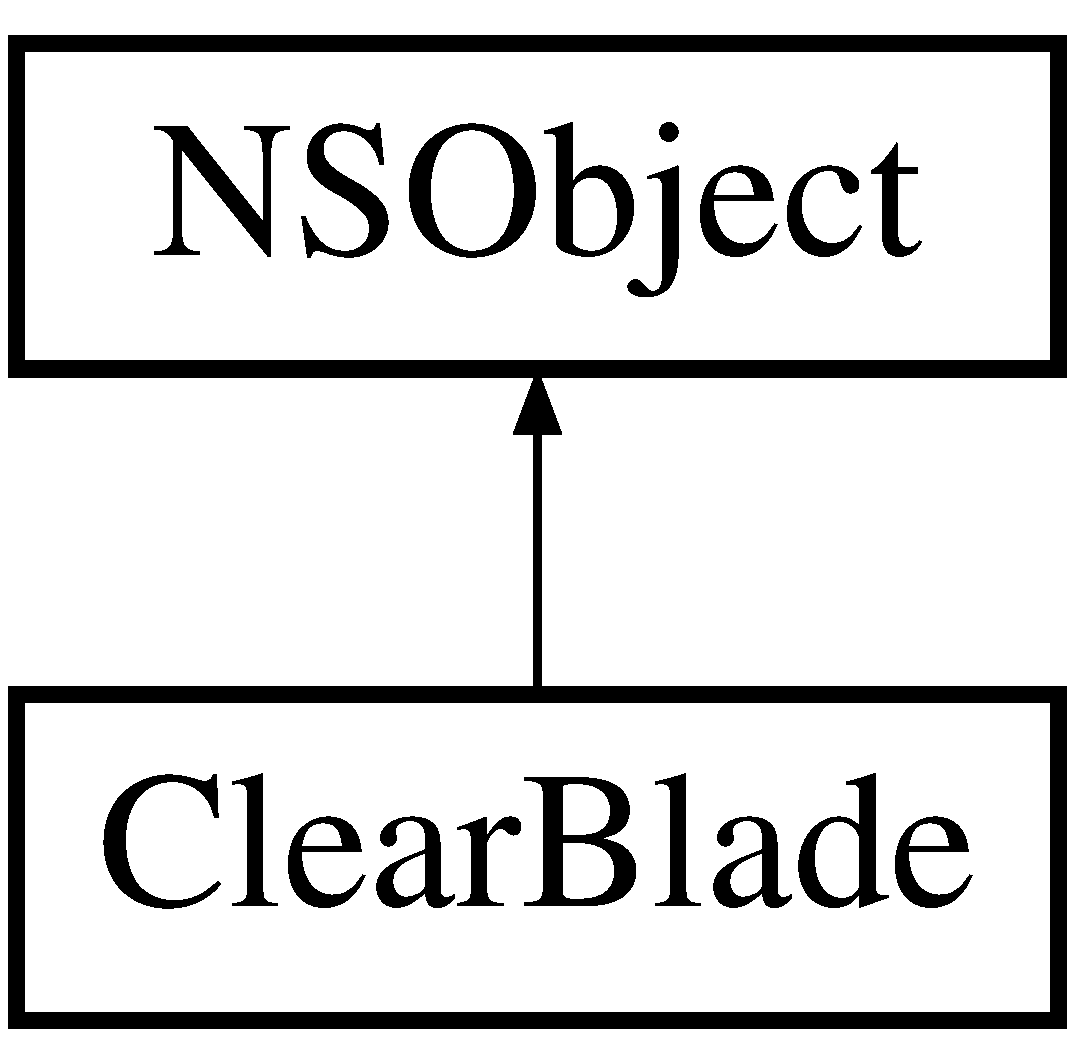
\includegraphics[height=2.000000cm]{interface_clear_blade}
\end{center}
\end{figure}
\subsection*{Instance Methods}
\begin{DoxyCompactItemize}
\item 
(void) -\/ \hyperlink{interface_clear_blade_a4a2da5ca59acd23e44d0f793e9eb778b}{log\+Error\+:}
\item 
(void) -\/ \hyperlink{interface_clear_blade_aa1d4699543bf38e300b5b0ad256c44c2}{log\+Warning\+:}
\item 
(void) -\/ \hyperlink{interface_clear_blade_ada4ef00171405d7247b1d07d3a3e70f6}{log\+Debug\+:}
\item 
(void) -\/ \hyperlink{interface_clear_blade_a03f35439a4d2b9908872cfdfbd50a0b5}{log\+Extra\+:}
\item 
(int) -\/ \hyperlink{interface_clear_blade_acdf4d6feb5a40c60be3b4ed0846d52e5}{generate\+I\+D}
\end{DoxyCompactItemize}
\subsection*{Class Methods}
\begin{DoxyCompactItemize}
\item 
(instancetype) + \hyperlink{interface_clear_blade_accced1239f531de87d166d617a021673}{settings}
\item 
(instancetype) + \hyperlink{interface_clear_blade_a234fefa317e73d46768506a34a89e5fa}{init\+Settings\+Sync\+With\+System\+Key\+:with\+System\+Secret\+:with\+Options\+:with\+Error\+:}
\item 
(void) + \hyperlink{interface_clear_blade_a76b3d3e815239c17dba4f858e774bcab}{init\+Settings\+With\+System\+Key\+:with\+System\+Secret\+:with\+Options\+:with\+Success\+Callback\+:with\+Error\+Callback\+:}
\end{DoxyCompactItemize}
\subsection*{Properties}
\begin{DoxyCompactItemize}
\item 
N\+S\+String $\ast$ \hyperlink{interface_clear_blade_aab0eaf0d5cb8cabae0889b19230859b5}{system\+Key}
\item 
N\+S\+String $\ast$ \hyperlink{interface_clear_blade_ac86550adaf64238807f4bc536af7d1d0}{system\+Secret}
\item 
N\+S\+String $\ast$ \hyperlink{interface_clear_blade_a254d692b3e85e4d33a4518e9ff9e4f40}{server\+Address}
\item 
N\+S\+U\+R\+L $\ast$ \hyperlink{interface_clear_blade_a6d90355650360ef27ac6aad5f3df2a7b}{messaging\+Address}
\item 
C\+B\+Message\+Client\+Quality \hyperlink{interface_clear_blade_a886dc9ea49818af85910b4373f95096b}{messaging\+Default\+Qo\+S}
\item 
\hyperlink{interface_c_b_user}{C\+B\+User} $\ast$ \hyperlink{interface_clear_blade_a2c5ec6113244b327a374c1f939efbce5}{main\+User}
\item 
C\+B\+Logging\+Level \hyperlink{interface_clear_blade_a63988be37c99a5e90c91b89be9106a5d}{logging\+Level}
\end{DoxyCompactItemize}


\subsection{Detailed Description}
Encapsulates all the global configuration for the \hyperlink{interface_clear_blade}{Clear\+Blade} A\+P\+I 

\subsection{Method Documentation}
\hypertarget{interface_clear_blade_acdf4d6feb5a40c60be3b4ed0846d52e5}{\index{Clear\+Blade@{Clear\+Blade}!generate\+I\+D@{generate\+I\+D}}
\index{generate\+I\+D@{generate\+I\+D}!Clear\+Blade@{Clear\+Blade}}
\subsubsection[{generate\+I\+D}]{\setlength{\rightskip}{0pt plus 5cm}-\/ (int) generate\+I\+D 
\begin{DoxyParamCaption}
{}
\end{DoxyParamCaption}
}}\label{interface_clear_blade_acdf4d6feb5a40c60be3b4ed0846d52e5}
Generates an I\+D that's guaranteed to be unique for this instance of \hyperlink{interface_clear_blade}{Clear\+Blade} Settings \hypertarget{interface_clear_blade_a234fefa317e73d46768506a34a89e5fa}{\index{Clear\+Blade@{Clear\+Blade}!init\+Settings\+Sync\+With\+System\+Key\+:with\+System\+Secret\+:with\+Options\+:with\+Error\+:@{init\+Settings\+Sync\+With\+System\+Key\+:with\+System\+Secret\+:with\+Options\+:with\+Error\+:}}
\index{init\+Settings\+Sync\+With\+System\+Key\+:with\+System\+Secret\+:with\+Options\+:with\+Error\+:@{init\+Settings\+Sync\+With\+System\+Key\+:with\+System\+Secret\+:with\+Options\+:with\+Error\+:}!Clear\+Blade@{Clear\+Blade}}
\subsubsection[{init\+Settings\+Sync\+With\+System\+Key\+:with\+System\+Secret\+:with\+Options\+:with\+Error\+:}]{\setlength{\rightskip}{0pt plus 5cm}+ (instancetype) init\+Settings\+Sync\+With\+System\+Key\+: 
\begin{DoxyParamCaption}
\item[{(N\+S\+String $\ast$)}]{key}
\item[{withSystemSecret:(N\+S\+String $\ast$)}]{secret}
\item[{withOptions:(N\+S\+Dictionary $\ast$)}]{options}
\item[{withError:(N\+S\+Error $\ast$$\ast$)}]{error}
\end{DoxyParamCaption}
}}\label{interface_clear_blade_a234fefa317e73d46768506a34a89e5fa}
Initializes settings synchronously with default settings. Also initializes with an anonymous user. 
\begin{DoxyParams}{Parameters}
{\em key} & The System Key. \\
\hline
{\em secret} & The System Secret. \\
\hline
{\em error} & Is set if the \hyperlink{interface_clear_blade}{Clear\+Blade} settings fails to initialize \\
\hline
\end{DoxyParams}
\begin{DoxyReturn}{Returns}
The newly created Settings object 
\end{DoxyReturn}
\hypertarget{interface_clear_blade_a76b3d3e815239c17dba4f858e774bcab}{\index{Clear\+Blade@{Clear\+Blade}!init\+Settings\+With\+System\+Key\+:with\+System\+Secret\+:with\+Options\+:with\+Success\+Callback\+:with\+Error\+Callback\+:@{init\+Settings\+With\+System\+Key\+:with\+System\+Secret\+:with\+Options\+:with\+Success\+Callback\+:with\+Error\+Callback\+:}}
\index{init\+Settings\+With\+System\+Key\+:with\+System\+Secret\+:with\+Options\+:with\+Success\+Callback\+:with\+Error\+Callback\+:@{init\+Settings\+With\+System\+Key\+:with\+System\+Secret\+:with\+Options\+:with\+Success\+Callback\+:with\+Error\+Callback\+:}!Clear\+Blade@{Clear\+Blade}}
\subsubsection[{init\+Settings\+With\+System\+Key\+:with\+System\+Secret\+:with\+Options\+:with\+Success\+Callback\+:with\+Error\+Callback\+:}]{\setlength{\rightskip}{0pt plus 5cm}+ (void) init\+Settings\+With\+System\+Key\+: 
\begin{DoxyParamCaption}
\item[{(N\+S\+String $\ast$)}]{key}
\item[{withSystemSecret:(N\+S\+String $\ast$)}]{secret}
\item[{withOptions:(N\+S\+Dictionary $\ast$)}]{options}
\item[{withSuccessCallback:(Clear\+Blade\+Settings\+Success\+Callback)}]{success\+Callback}
\item[{withErrorCallback:(Clear\+Blade\+Settings\+Error\+Callback)}]{error\+Callback}
\end{DoxyParamCaption}
}}\label{interface_clear_blade_a76b3d3e815239c17dba4f858e774bcab}
Initializes settings asynchronously with default settings. Also initializes with an anonymous user. 
\begin{DoxyParams}{Parameters}
{\em key} & The System Key. \\
\hline
{\em secret} & The System Secret. \\
\hline
{\em success\+Callback} & The callback for when settings successfully initializes. \\
\hline
{\em error\+Callback} & The callback for when settings fails to initialize for whatever reason \\
\hline
\end{DoxyParams}
\hypertarget{interface_clear_blade_ada4ef00171405d7247b1d07d3a3e70f6}{\index{Clear\+Blade@{Clear\+Blade}!log\+Debug\+:@{log\+Debug\+:}}
\index{log\+Debug\+:@{log\+Debug\+:}!Clear\+Blade@{Clear\+Blade}}
\subsubsection[{log\+Debug\+:}]{\setlength{\rightskip}{0pt plus 5cm}-\/ (void) log\+Debug\+: 
\begin{DoxyParamCaption}
\item[{(N\+S\+String $\ast$)}]{debug}
\item[{,}]{...}
\end{DoxyParamCaption}
}}\label{interface_clear_blade_ada4ef00171405d7247b1d07d3a3e70f6}
Logs a debug statement as filtered by the logging\+Level setting \hypertarget{interface_clear_blade_a4a2da5ca59acd23e44d0f793e9eb778b}{\index{Clear\+Blade@{Clear\+Blade}!log\+Error\+:@{log\+Error\+:}}
\index{log\+Error\+:@{log\+Error\+:}!Clear\+Blade@{Clear\+Blade}}
\subsubsection[{log\+Error\+:}]{\setlength{\rightskip}{0pt plus 5cm}-\/ (void) log\+Error\+: 
\begin{DoxyParamCaption}
\item[{(N\+S\+String $\ast$)}]{error}
\item[{,}]{...}
\end{DoxyParamCaption}
}}\label{interface_clear_blade_a4a2da5ca59acd23e44d0f793e9eb778b}
Logs an error as filtered by the logging\+Level setting \hypertarget{interface_clear_blade_a03f35439a4d2b9908872cfdfbd50a0b5}{\index{Clear\+Blade@{Clear\+Blade}!log\+Extra\+:@{log\+Extra\+:}}
\index{log\+Extra\+:@{log\+Extra\+:}!Clear\+Blade@{Clear\+Blade}}
\subsubsection[{log\+Extra\+:}]{\setlength{\rightskip}{0pt plus 5cm}-\/ (void) log\+Extra\+: 
\begin{DoxyParamCaption}
\item[{(N\+S\+String $\ast$)}]{extra}
\item[{,}]{...}
\end{DoxyParamCaption}
}}\label{interface_clear_blade_a03f35439a4d2b9908872cfdfbd50a0b5}
Logs a extra data as filtered by the logging\+Level setting \hypertarget{interface_clear_blade_aa1d4699543bf38e300b5b0ad256c44c2}{\index{Clear\+Blade@{Clear\+Blade}!log\+Warning\+:@{log\+Warning\+:}}
\index{log\+Warning\+:@{log\+Warning\+:}!Clear\+Blade@{Clear\+Blade}}
\subsubsection[{log\+Warning\+:}]{\setlength{\rightskip}{0pt plus 5cm}-\/ (void) log\+Warning\+: 
\begin{DoxyParamCaption}
\item[{(N\+S\+String $\ast$)}]{warning}
\item[{,}]{...}
\end{DoxyParamCaption}
}}\label{interface_clear_blade_aa1d4699543bf38e300b5b0ad256c44c2}
Logs a warning as filtered by the logging\+Level setting \hypertarget{interface_clear_blade_accced1239f531de87d166d617a021673}{\index{Clear\+Blade@{Clear\+Blade}!settings@{settings}}
\index{settings@{settings}!Clear\+Blade@{Clear\+Blade}}
\subsubsection[{settings}]{\setlength{\rightskip}{0pt plus 5cm}+ (instancetype) settings 
\begin{DoxyParamCaption}
{}
\end{DoxyParamCaption}
}}\label{interface_clear_blade_accced1239f531de87d166d617a021673}
The global settings used by queries by default 

\subsection{Property Documentation}
\hypertarget{interface_clear_blade_a63988be37c99a5e90c91b89be9106a5d}{\index{Clear\+Blade@{Clear\+Blade}!logging\+Level@{logging\+Level}}
\index{logging\+Level@{logging\+Level}!Clear\+Blade@{Clear\+Blade}}
\subsubsection[{logging\+Level}]{\setlength{\rightskip}{0pt plus 5cm}-\/ (C\+B\+Logging\+Level) logging\+Level\hspace{0.3cm}{\ttfamily [read]}, {\ttfamily [write]}, {\ttfamily [atomic]}, {\ttfamily [assign]}}}\label{interface_clear_blade_a63988be37c99a5e90c91b89be9106a5d}
The Logging level the A\+P\+I uses. Defaults to C\+B\+\_\+\+L\+O\+G\+\_\+\+W\+A\+R\+N \hypertarget{interface_clear_blade_a2c5ec6113244b327a374c1f939efbce5}{\index{Clear\+Blade@{Clear\+Blade}!main\+User@{main\+User}}
\index{main\+User@{main\+User}!Clear\+Blade@{Clear\+Blade}}
\subsubsection[{main\+User}]{\setlength{\rightskip}{0pt plus 5cm}-\/ ({\bf C\+B\+User}$\ast$) main\+User\hspace{0.3cm}{\ttfamily [read]}, {\ttfamily [write]}, {\ttfamily [atomic]}, {\ttfamily [strong]}}}\label{interface_clear_blade_a2c5ec6113244b327a374c1f939efbce5}
The Main User of the app. Can be modified at runtime to change main users \hypertarget{interface_clear_blade_a6d90355650360ef27ac6aad5f3df2a7b}{\index{Clear\+Blade@{Clear\+Blade}!messaging\+Address@{messaging\+Address}}
\index{messaging\+Address@{messaging\+Address}!Clear\+Blade@{Clear\+Blade}}
\subsubsection[{messaging\+Address}]{\setlength{\rightskip}{0pt plus 5cm}-\/ (N\+S\+U\+R\+L$\ast$) messaging\+Address\hspace{0.3cm}{\ttfamily [read]}, {\ttfamily [atomic]}, {\ttfamily [assign]}}}\label{interface_clear_blade_a6d90355650360ef27ac6aad5f3df2a7b}
The Address for the Platform messaging service \hypertarget{interface_clear_blade_a886dc9ea49818af85910b4373f95096b}{\index{Clear\+Blade@{Clear\+Blade}!messaging\+Default\+Qo\+S@{messaging\+Default\+Qo\+S}}
\index{messaging\+Default\+Qo\+S@{messaging\+Default\+Qo\+S}!Clear\+Blade@{Clear\+Blade}}
\subsubsection[{messaging\+Default\+Qo\+S}]{\setlength{\rightskip}{0pt plus 5cm}-\/ (C\+B\+Message\+Client\+Quality) messaging\+Default\+Qo\+S\hspace{0.3cm}{\ttfamily [read]}, {\ttfamily [atomic]}, {\ttfamily [assign]}}}\label{interface_clear_blade_a886dc9ea49818af85910b4373f95096b}
The Default quality of service to use for messaging clients \hypertarget{interface_clear_blade_a254d692b3e85e4d33a4518e9ff9e4f40}{\index{Clear\+Blade@{Clear\+Blade}!server\+Address@{server\+Address}}
\index{server\+Address@{server\+Address}!Clear\+Blade@{Clear\+Blade}}
\subsubsection[{server\+Address}]{\setlength{\rightskip}{0pt plus 5cm}-\/ (N\+S\+String$\ast$) server\+Address\hspace{0.3cm}{\ttfamily [read]}, {\ttfamily [atomic]}, {\ttfamily [assign]}}}\label{interface_clear_blade_a254d692b3e85e4d33a4518e9ff9e4f40}
The Address for the Platform Data service \hypertarget{interface_clear_blade_aab0eaf0d5cb8cabae0889b19230859b5}{\index{Clear\+Blade@{Clear\+Blade}!system\+Key@{system\+Key}}
\index{system\+Key@{system\+Key}!Clear\+Blade@{Clear\+Blade}}
\subsubsection[{system\+Key}]{\setlength{\rightskip}{0pt plus 5cm}-\/ (N\+S\+String$\ast$) system\+Key\hspace{0.3cm}{\ttfamily [read]}, {\ttfamily [atomic]}, {\ttfamily [assign]}}}\label{interface_clear_blade_aab0eaf0d5cb8cabae0889b19230859b5}
The System Key used throughout the A\+P\+I \hypertarget{interface_clear_blade_ac86550adaf64238807f4bc536af7d1d0}{\index{Clear\+Blade@{Clear\+Blade}!system\+Secret@{system\+Secret}}
\index{system\+Secret@{system\+Secret}!Clear\+Blade@{Clear\+Blade}}
\subsubsection[{system\+Secret}]{\setlength{\rightskip}{0pt plus 5cm}-\/ (N\+S\+String$\ast$) system\+Secret\hspace{0.3cm}{\ttfamily [read]}, {\ttfamily [atomic]}, {\ttfamily [assign]}}}\label{interface_clear_blade_ac86550adaf64238807f4bc536af7d1d0}
The System Secret used throughout the A\+P\+I 

The documentation for this class was generated from the following file\+:\begin{DoxyCompactItemize}
\item 
Clear\+Blade\+A\+P\+I/Clear\+Blade.\+h\end{DoxyCompactItemize}

\hypertarget{category_clear_blade_07_08}{\section{Clear\+Blade() Category Reference}
\label{category_clear_blade_07_08}\index{Clear\+Blade()@{Clear\+Blade()}}
}
\subsection*{Instance Methods}
\begin{DoxyCompactItemize}
\item 
\hypertarget{category_clear_blade_07_08_a0d43815879fb0a4b769552ac24e08826}{(instancetype) -\/ {\bfseries init\+With\+System\+Key\+:with\+System\+Secret\+:with\+Options\+:}}\label{category_clear_blade_07_08_a0d43815879fb0a4b769552ac24e08826}

\end{DoxyCompactItemize}
\subsection*{Properties}
\begin{DoxyCompactItemize}
\item 
\hypertarget{category_clear_blade_07_08_aaf2f0eda9ee883fbd5e6e152579c9dc9}{N\+S\+Number $\ast$ {\bfseries next\+I\+D}}\label{category_clear_blade_07_08_aaf2f0eda9ee883fbd5e6e152579c9dc9}

\item 
\hypertarget{category_clear_blade_07_08_a88ac8ac01e37d365cbac7227e738bf40}{C\+B\+Message\+Client\+Quality {\bfseries messaging\+Default\+Qo\+S}}\label{category_clear_blade_07_08_a88ac8ac01e37d365cbac7227e738bf40}

\end{DoxyCompactItemize}


The documentation for this category was generated from the following file\+:\begin{DoxyCompactItemize}
\item 
Clear\+Blade\+A\+P\+I/Clear\+Blade.\+m\end{DoxyCompactItemize}

%--- End generated contents ---

% Index
\newpage
\phantomsection
\addcontentsline{toc}{chapter}{Index}
\printindex

\end{document}
